\chapter{\chatextprobReasoning}\label{cha:probReasoning}

After having investigated sparse decomposition schemes of probability distributions into tensor networks, we now exploit these schemes to derive efficient reasoning schemes. % Start of Focus Reasoning here
We first introduce by queries a generic scheme to retrieve information by contractions, and introduce the method of maximum likelihood estimation related to entropy optimization.
Then we focus on inference tasks in exponential families, which have been introduced as a generalization of graphical models in the previous chapter.


\sect{Queries}

The efficient retrieval of information stored in probability distributions has to exploit the available decomposition schemes.
To avoid the instantiation of a distribution based on its decomposition, we directly define deductive reasoning schemes by contractions, which can be executed using the available decomposition.

\subsect{Querying by functions}

We now formalize queries by retrieving expectations of functions given a distribution specified by probability tensors.
We exploit basis calculus in defining categorical variables $\headvariableof{\exfunction}$ to tensors $\exfunction$, which are enumerating the set $\imageof{\exfunction}$.
More details on this scheme are provided in \charef{cha:basisCalculus}, see \defref{def:functionRelationEncoding} therein.

\begin{definition}
    \label{def:queries}
    The marginal query of a probability distribution $\probat{\shortcatvariables}$ by a query statistic
    \begin{align*}
        \exfunction : \facstates \rightarrow \arbsetof{\exfunction}
    \end{align*}
    is the vector $\probat{\headvariableof{\exfunction}}$, where $\headvariableof{\exfunction}$ is an image enumerating variable (see \charef{cha:basisCalculus} for more details), defined as the contraction
    \begin{align*}
        \probat{\headvariableof{\exfunction}}
        = \contractionof{\probat{\shortcatvariables},\rencodingofat{\exfunction}{\headvariableof{\exfunction},\shortcatvariables}}{\headvariableof{\exfunction}} \, .
    \end{align*}
    If $\arbsetof{\exfunction}\subset\rr$, and the statistic $\exfunction$ is therefore a tensor, we further define the expectation query of $\probwith$ by $\exfunction$ as
    \begin{align*}
        \expectationof{\exfunction} = \sbcontraction{\exfunctionat{\shortcatvariables},\probwith} \, .
    \end{align*}
    Given another query statistic $\secexfunction: \facstates \rightarrow \arbsetof{\secexfunction}$, which image is enumerated by a variable $\headvariableof{\secexfunction}$, the conditional query of the probability distribution $\probat{\shortcatvariables}$ by the statistic $\exfunction$ conditioned on $\secexfunction$ is the matrix $\condprobof{\headvariableof{\exfunction}}{\headvariableof{\secexfunction}}\in\rr^{\cardof{\imageof{\exfunction}}}\otimes \rr^{\cardof{\imageof{\secexfunction}}}$ defined as the normation
    \begin{align*}
        \condprobof{\headvariableof{\exfunction}}{\headvariableof{\secexfunction}}
        = \normationofwrt{
            \probat{\shortcatvariables},\rencodingofat{\exfunction}{\headvariableof{\exfunction},\shortcatvariables},\rencodingofat{\secexfunction}{\headvariableof{\secexfunction},\shortcatvariables}
        }{
            \headvariableof{\exfunction}}{\headvariableof{\secexfunction}
        } \, .
    \end{align*}
\end{definition}

We notice, that marginal and conditional queries generalize the schemes of marginalization and conditioning on the distributed variables.
As such, marginal distributions are marginal queries with respect to a identity query statistic acting on the respective variables.
Conditional distributions can be similarly retrieved by two identity statistics, representing the incoming and outgoing variables.
%The query framework of \defref{def:queries} can be used beyond marginal and conditional quereis for the customized information retrieval.

%% Relation of queries and expectation queries
Expectation queries return the expectation of a real-valued feature $\exfunction : \facstates\rightarrow\rr$.
When understanding $\exfunction$ as a random variable given the probability measure $\probat{\shortcatvariables}$, the expectation query returns the expectation of that random variable.
Expectation queries are further contractions of marginal queries with the identity function restricted on the image of $\exfunction$, since
\begin{align*}
    \expectationof{\exfunction}
    = \contraction{\probat{\headvariableof{\exfunction}},\idrestrictedto{\imageof{\exfunction}}{\headvariableof{\exfunction}} } \, .
\end{align*}
This contraction equations follows from the more general \corref{cor:rhoToNormal}, which will be shown in \charef{cha:basisCalculus}.
\red{Expectation queries on statistics build the mean parameter of a distribution.}

%% Conditional Probabilities and conditional queries
%Conditional probabilities are queries, where the tensors $\exfunction$ and $\secexfunction$ are identity mappings in the respective variable state spaces.
%Conversely, we can understand the conditional query $\condprobof{\headvariableof{\exfunction}}{\headvariableof{\secexfunction}}$ as the conditional probability of a query statistic $\exfunction$ conditioned on $\secexfunction$, of the underlying Markov Network with cores $\{\probtensor, \rencodingof{\exfunction}, \rencodingof{\secexfunction} \}$ and variables $\catvariableof{\exfunction},\catvariableof{\secexfunction}$ besides the variables distributed by $\probtensor$.

%%% Expectations as event queries -> Consistency with $\probat{X=i}$?
%We further denote event queries by
%	\[  \expectationof{\exfunction=\exfunctionimageelement} = \sbcontraction{\probtensor,\rencodingof{\exfunction},\onehotmapof{\exfunctionimageelement}}\]
%where by $\onehotmapof{z}$ be denote the one hot encoding of the state $z$ with respect to some enumeration.
%Let us note that they are further contraction of the queries in \defref{def:queries} since by \theref{the:splittingContractions}
%\begin{align*}
%	 \expectationof{\exfunction=z}
%	& =  \sbcontraction{ \sbcontractionof{\probtensor,\rencodingof{\exfunction}}{\catvariableof{\exfunction}} ,\onehotmapof{z}}\\
%	& =  \sbcontraction{ \probat{\exfunction} ,\onehotmapof{z}} \, .
%\end{align*}

\subsect{Mode Queries}\label{sec:modeQueries}

A different kind of queries are mode queries, which we formalize by the searches of the indices to maximal coordinates in a tensor.

\begin{definition}
    Given a tensor $\hypercorewith$ the mode query is the problem
    \begin{align}
        \argmax_{\shortcatindicesin} \hypercoreat{\indexedshortcatvariables} \, .
    \end{align}
\end{definition}

%MAP relation - Needed?
%Mode queries are often called MAP queries.
%The name MAP is an abbreviation of maximum a-posteriori, since it searches for the most probable state in probability distributions.
%The term a-posteriori originates from a focus on conditional probabilities, which slices with respect to incoming variables represent the a-posteriori distribution given evidence on the incoming variables.
%We will in this work use this term for generic maximum coordinate searches.

% Convex optimization
We can pose mode queries as convex optimization problems.
To this end we recall, that the set of all probability distributions is a convex hull of the one-hot encoded states, that is
\begin{align*}
    \bmrealprobof{\ones}
    = \convhullof{\onehotmapofat{\shortcatindices}{\shortcatvariables} \, : \, \shortcatindicesin} \, .
\end{align*}
With this we have
\begin{align*}
    \max_{\shortcatindices} \hypercoreat{\indexedshortcatvariables}
    &= \max_{\shortcatindices} \contraction{\hypercoreat{\shortcatvariables},\onehotmapofat{\shortcatindices}{\shortcatvariables}} \\
    &= \max_{\meanparamat{\shortcatvariables}\in\bmrealprobof{\ones}} \contraction{\hypercoreat{\shortcatvariables},\meanparamat{\shortcatvariables}} \, .
\end{align*}
We note that the maximation over $\bmrealprobof{\ones}$ is a convex optimization problem and the maxima are taken at
\begin{align*}
    \argmax_{\meanparamat{\shortcatvariables}\in\bmrealprobof{\ones}} \contraction{\hypercoreat{\shortcatvariables},\meanparamat{\shortcatvariables}}
    = \convhullof{\onehotmapofat{\shortcatindices}{\shortcatvariables} \, : \, \shortcatindices\in\argmax_{\shortcatindices} \hypercoreat{\indexedshortcatvariables}} \, .
\end{align*}
We will further apply this generic trick to approach mode queries when studying inference problems for exponential families in the following sections.

% Restriction to subsets
Let us note, that we can also approach modified mode queries, where we restrict to $\arbset\subset\facstates$, namely
\begin{align*}
    \argmax_{\shortcatindices\in\arbset} \hypercoreat{\indexedshortcatvariables} \, .
\end{align*}
We can choose the base measure by the subset encoding (see \charef{cha:basisCalculus}) of $\arbset$, namely
\begin{align*}
    \basemeasurewith = \sum_{\shortcatindices\in\arbset} \onehotmapofat{\shortcatindices}{\shortcatvariables} \, ,
\end{align*}
and conclude that
\begin{align*}
    \argmax_{\meanparamat{\shortcatvariables}\in\bmrealprobof{\basemeasure}} \contraction{\hypercoreat{\shortcatvariables},\meanparamat{\shortcatvariables}}
    = \convhullof{\onehotmapofat{\shortcatindices}{\shortcatvariables} \, : \, \shortcatindices\in\argmax_{\shortcatindices\in\arbset} \hypercoreat{\indexedshortcatvariables}} \, .
\end{align*}



\subsect{Energy representations}

For exponential families (see \secref{sec:exponentialFamilies}) we have observed, that often energy tensors have feasible tensor network representations, whereas the corresponding probability distributions can get infeasible.
We therefore investigate here schemes to answer queries based on the energy tensor instead of the distribution.
%Let us now interpret a probability tensor at hand as a member of an exponential family (see \secref{sec:exponentialFamilies}), which is always possible when taking the naive exponential family.

\begin{theorem}
    \label{the:energyContractionQueries} % This is a statement about "full" queries.
    Let $\energytensorat{\shortcatvariables}$ be an energy tensor and $\probwith=\normationof{\expof{\energytensorat{\shortcatvariables}}}{\shortcatvariables}$ the corresponding distribution.
%	For any probability distribution $\probtensor$ with $\probtensor= \normationof{\expof{\energytensorat{\shortcatvariables}}}{\shortcatvariables}$,
    For disjoint subsets $\nodesa,\nodesb \subset [\catorder]$ with $\nodesa\cup\nodesb=[\catorder]$ and any $\catindexof{\nodesb}$ we have
    \begin{align*}
        \condprobof{\catvariableof{\nodesa}}{\indexedcatvariableof{\nodesb}}
        = \normationof{
            \expof{\energytensorat{\catvariableof{\nodesa},\indexedcatvariableof{\nodesb}}}
        }{\catvariableof{\nodesa}} \, .
    \end{align*}
\end{theorem}
\begin{proof}
    To show the theorem, we use a generic simplification property of coordinatewise transforms, which we will show as \lemref{lem:coordinatewisetrafoSliceReduction} in \charef{cha:coordinateCalculus} and get
    \begin{align*}
        \contractionof{\expof{\energytensorat{\catvariableof{\nodesa},\catvariableof{\nodesb}}}}{\catvariableof{\nodesa},\indexedcatvariableof{\nodesb}}
        = \contractionof{\expof{\energytensorat{\catvariableof{\nodesa},\indexedcatvariableof{\nodesb}}}}{\catvariableof{\nodesa}}
    \end{align*}
    Based on this we get
    \begin{align*}
        \condprobof{\catvariableof{\nodesa}}{\indexedcatvariableof{\nodesb}}
        = \normationofwrt{\expof{\energytensorat{\catvariableof{\nodesa},\catvariableof{\nodesb}}}}{\catvariableof{\nodesa}}{\indexedcatvariableof{\nodesb}} \\
        = \frac{\contractionof{\expof{\energytensorat{\catvariableof{\nodesa},\catvariableof{\nodesb}}}}{\catvariableof{\nodesa},\indexedcatvariableof{\nodesb}}}{
            \contractionof{\expof{\energytensorat{\catvariableof{\nodesa},\catvariableof{\nodesb}}}}{\indexedcatvariableof{\nodesb}}
        } \\
        = \frac{\contractionof{\expof{\energytensorat{\catvariableof{\nodesa},\indexedcatvariableof{\nodesb}}}}{\catvariableof{\nodesa}}}{
            \contraction{\expof{\energytensorat{\catvariableof{\nodesa},\indexedcatvariableof{\nodesb}}}}
        } \\
        = \normationof{
            \expof{\energytensorat{\catvariableof{\nodesa},\indexedcatvariableof{\nodesb}}}
        }{\catvariableof{\nodesa}} \, .
    \end{align*}
\end{proof}

% Situation of marginalized variables
Importantly, \theref{the:energyContractionQueries} does not generalize to situations, where $\nodesa\cup\nodesb\neq[\catorder]$, since summation over the indices of the variables $[\catorder]/\nodesa\cup\nodesb$ and contraction do not commute.
In this more generic situation, we would need to sum over exponentiated coordinates, that is
\begin{align*}
    \condprobof{\catvariableof{\nodesa}}{\indexedcatvariableof{\nodesb}}
    = \normationof{
        \sum_{\catindexofin{[\catorder]/\nodesa\cup\nodesb}}
        \expof{\energytensorat{\catvariableof{\nodesa},\indexedcatvariableof{\nodesb},\indexedcatvariableof{[\catorder]/\nodesa\cup\nodesb}}}
    }{\catvariableof{\nodesa}} \, .
\end{align*}


% Mode queries
Mode queries on probability distributions in an energy representation can always be reduces to mode queries on the energy tensor.
This is due to the monotonicity of the exponential function, which implies
\begin{align*}
    \argmax_{\shortcatindicesin} \probat{\indexedshortcatvariables}
    &=\argmax_{\shortcatindicesin} \normationof{\expof{\energytensorat{\shortcatvariables}}}{\indexedshortcatvariables} \\
    &=\argmax_{\shortcatindicesin} \expof{\energytensorat{\indexedshortcatvariables}} \\
    &=\argmax_{\shortcatindicesin} \energytensorat{\indexedshortcatvariables} \, .
\end{align*}
Since we are only interested in identifying the index of the maximum coordinate, and not its value, we have further dropped the normalization term by partition functions.
When one instead need to get the value of the maximal, the partition function cannot be ignored.

\sect{Sampling}

Let us here investigate how to draw samples from a prbability distribution, based on queries on it.
Naive methods, such as drawing a random number in $[0,1]$, adding iteratively the coordinates and stopping when the sum exceeds the random variables, are infeasible when having large tensor orders causing exponential increases of the coordinate number.
We recall, that the number of coordinates of $\probwith$ is $\prod_{\catenumeratorin}\catdimof{\catenumerator}$, which increases exponentially in the number $\catorder$ of the variables.
Efficient methods instead have to exploit tensor network decompositions of the decompositions.

\subsect{Exact Methods}

The first insight to derive efficient sampling algorithms is to sample a single variable in each step.
Forward sampling (see \algoref{alg:ForwardSampling}) exploits to this end the generic chain decomposition (see \theref{the:chainRule}) of a probability distribution, namely
\begin{align*}
    \probwith = \contractionof{\{\margprobat{\catvariableof{0}}\} \cup
    \left\{\condprobof{\catvariableof{\catenumerator}}{\catvariableof{0},\ldots,\catvariableof{\catenumerator-1}}\,:\,\catenumeratorin, \, \catenumerator\geq 1\right\}
    }{\shortcatvariables} \, ,
\end{align*}
It then samples iteratively a state $\catindexof{\catenumerator}$ for the variable $\catvariableof{\catenumerator}$ conditioned on the previously sampled states, that is from the conditonal distribution
\begin{align*}
    \condprobof{\catvariableof{\catenumerator}}{\indexedcatvariableof{[\catenumerator]}} \, .
\end{align*}
The generic chain decomposition thereby ensures that probability of getting a state $\shortcatindices$ by this procedure coincides with $\probat{\indexedshortcatvariables}$.

\begin{algorithm}[hbt!]
    \caption{Forward Sampling}\label{alg:ForwardSampling}
    \begin{algorithmic}
        \Require Probability distribution $\probtensor$
        \Ensure Exact sample $\catindices$ of $\probtensor$
        \hrule
        \For{$\catenumeratorin$}
            \State Draw $\catindexof{\catenumerator}\in[\catdimof{\catenumerator}]$ from the conditional distribution
            \begin{align*}
                \condprobof{\catvariableof{\catenumerator}}{\indexedcatvariableof{[\catenumerator]}}
            \end{align*}
        \EndFor
    \end{algorithmic}
\end{algorithm}

% Bayesian networks
Forward Sampling is especially efficient, when sampling from a Bayesian Network respecting the topological order of its nodes.
More technically, when the parents $\parentsof{\catenumerator}$ of a node $\catenumerator$ are contained in the preceding variables $[\catenumerator]$, we apply the conditional independence assumption (more precisely \theref{the:conditionDropping} in combination with \theref{the:condIndBN}) to get
\begin{align*}
    \condprobof{\catvariableof{\catenumerator}}{\indexedcatvariableof{[\catenumerator]}}
    = \condprobof{\catvariableof{\catenumerator}}{\indexedcatvariableof{\parentsof{\catenumerator}}} \, .
\end{align*}
Since this conditional probability coincides with a local tensor in the Bayesian Network, we can avoid to contract the network for preparing the conditional distribution.
Different to more general Markov Networks, forward sampling from Bayesian Network can therefore be done efficiently by reduction to conditional queries answerable using local tensors.
We note that it is important to sample in the topological order induced by the underlying directed hypergraph, since the computation of generic conditional distributions is also for Bayesian Networks $\mathsf{NP}$-hard (see Chapter~13 in \cite{koller_probabilistic_2009}).
Sampling along the topological variable order requires only tractable to answer conditional queries on the Bayesian Network.

%% Comment on rejection Sampling 
%When sampling from conditional probability distributions, one can sample from the conditioned distribution instead.
%However, the conditioning changes the structure of the distribution, and conditioned Bayesian Networks are not Bayesian Networks on the same graph.
%One ways around is rejection sampling, where one samples from the unconditioned distribution and rejects samples not satisfying the event conditioned on.
%When the event conditioned on is of small probability, methods like rejection sampling will come with large runtimes.

\subsect{Gibbs Sampling}

While we have seen that forward sampling can be performed efficiently on Bayesian Networks, Gibbs sampling can be also performed efficiently for Markov Networks.
Gibbs sampling \algoref{alg:Gibbs} overcomes the intractability problems of sampling steps during forward sampling at the expense of repetitions of the sampling step.
%The tractability of each sampling step is traded off against the number of repetitions to produce a sample.
When performing finite repetitions, Gibbs sampling in general samples from an approximate distribution to the one desired.
It can be shown, that these approximate distribution tend to one desired in the asymptotic limit of infinite repetitions of the sampling step (see Chapter~12 in \cite{koller_probabilistic_2009}).

\begin{algorithm}[hbt!]
    \caption{Gibbs Sampling}\label{alg:Gibbs}
    \begin{algorithmic}
        \Require Probability distribution $\probtensor$
        \Ensure Approximative sample $\catindices$ of $\probtensor$
        \hrule
        \For{$\catenumeratorin$}
            \State Draw $\catindexof{\catenumerator}$ from an initialization distribution. % In implementation: Initialize with ones and draw -> Avoids zero probability state
        \EndFor
        \While{Stopping criterion is not met}
            \For{$\catenumeratorin$}
                \State Draw $\catindexof{\catenumerator}$ from the conditional distribution
                \begin{align*}
                    \condprobof{\catvariableof{\catenumerator}}{\indexedcatvariableof{[\catorder]/\{\catenumerator\}}}
                \end{align*}
            \EndFor
        \EndWhile
        \Return $\catindices$
    \end{algorithmic}
\end{algorithm}

% Efficiency on Markov Networks
The central problem of forward sampling on Markov Networks has been the need for global contractions to answer the required conditional queries, which originates from large numbers of variables to be marginalized out.
When avoiding the marginalization of variables, and conditioning on them instead, global contractions can be avoided.
To be more precise, for any tensor network $\extnet$ on $\graph=([\catorder],\edges)$ and any $\catenumeratorin$ we have
\begin{align*}
    \contractionof{\extnet}{\catvariableof{\catenumerator},\catvariableof{[\catorder]/\{\catenumerator\}}}
    = \contractionof{\{\hypercoreat{\edge}{\catvariableof{\catenumerator},\indexedcatvariableof{\edge/\{\catenumerator\}}} \, : \, \edge\in\edges, \, \catenumerator\in\edge\}}{\catvariableof{\catenumerator}}
    \cdot \prod_{\edge\in\edges, \, \catenumerator\notin\edge} \hypercoreat{\edge}{\indexedcatvariableof{\edge}} \, .
\end{align*}
As a consequence, we get for the Markov Network $\probtensor=\probof{\graph}$ to $\extnet$, that
\begin{align*}
    \condprobof{\catvariableof{\catenumerator}}{\indexedcatvariableof{[\catorder]/\{\catenumerator\}}}
    &= \normationof{\extnet}{\catvariableof{\catenumerator},\catvariableof{[\catorder]/\{\catenumerator\}}} \\
    &= \normationof{\{\hypercoreat{\edge}{\catvariableof{\catenumerator},\indexedcatvariableof{\edge/\{\catenumerator\}}} \, : \, \edge\in\edges, \, \catenumerator\in\edge\}}{\catvariableof{\catenumerator}} \, .
\end{align*}
The conditional queries on a Markov Network asked in Gibbs Sampling can therefore be answered by contractions only of those tensors containing the variable $\catvariableof{\catenumerator}$.
To find further locally answerable conditional queries, we need to condition only on the neighbored variables, refered to as Markov blanket, such that the other variables are conditionally independent.
This follows from the characterization of the conditional independences eminent in Markov Networks, which has been shown in \theref{the:condIndMN}, and can be used to design further tractable sampling schemes for Markov Networks.

% Energy
We can further answer these conditional queries efficiently, when we perform Gibbs sampling on a probability distribution in an energy representation, that is $\probwith=\normationof{\expof{\energytensorat{\shortcatvariables}}}{\shortcatvariables}$.
Using \theref{the:energyContractionQueries}, we have
\begin{align*}
    \condprobof{\catvariableof{\catenumerator}}{\indexedcatvariableof{[\catorder]/\{\catenumerator\}}}
    = \normationof{\expof{\energytensorat{\catvariableof{\catenumerator},\indexedcatvariableof{[\catorder]/\{\catenumerator\}}}}
    }{\catvariableof{\nodesa}}
\end{align*}
We note, that the main property of the conditional query exploited here, is that all variables but the one sampled appear as a condition and none is marginalized out.
In the scheme of forward sampling, where most of the variables are marginalized out in many queries, we cannot apply this trick and would have to perform sums over exponentiated coordinates to the variables marginalized out.


\subsect{Simulated Annealing}\label{sec:simulatedAnnealing}

Simulated annealing is an adapted sampling scheme that targets mode queries rather than generating representative samples from a distribution.
It employs an annealing process that gradually transforms the probability distribution by increasingly favoring high-likelihood configurations, thereby improving the chances of sampling a solution to a mode query.
To be more precise, let there be a distribution in energy representation, that is $\probwith=\normationof{\expof{\energytensorat{\shortcatvariables}}}{\shortcatvariables}$.
Whe introduce a parameter $\invtemp\in\rr$, which we understand as the inverse temperature, and anneal the distribution through scaling its energy by this parameter.
%\begin{align*}
%    \energytensorofat{\invtemp}{\shortcatvariables} = \invtemp \cdot \energytensorat{\shortcatvariables} \, .
%\end{align*}
In the limit of $\invtemp\rightarrow\infty$, for each state $\shortcatindicesin$ the annealed distribution behaves as
\begin{align*}
    \normationof{\expof{\invtemp\cdot\energytensorofat{\shortcatvariables}}}{\indexedshortcatvariables} \rightarrow
    \normationof{\ones_{\argmax_{\shortcatindicesin}\energytensorat{\indexedshortcatvariables}}}{\indexedshortcatvariables} \, .
\end{align*}
In this limit, the annealed distribution tends to the uniform distribution of the maximal coordinates, that is the uniform distribution of the set
\begin{align*}
    \argmax_{\shortcatindicesin}\energytensorat{\indexedshortcatvariables} = \argmax_{\shortcatindicesin}\probat{\indexedshortcatvariables} \, .
\end{align*}
i
To integrate annealing into Gibbs sampling, one chooses a parameter $\invtemp$ for each repetition of a sampling step and sample from the conditioned annealed distribution $\normationof{\expof{\invtemp\cdot\energytensorat{\shortcatvariables}}}{\shortcatvariables}$.
Through increasing $\invtemp$ during the algorithm, the samples are drawn towards states with larger coordinates in $\probat{\shortcatvariables}$.
However, when $\invtemp$ is large, the sampling procedure can get stuck in local maxima, whereas small $\invtemp$ are in favor of overcoming such.
The inverse temperature is thus understood as a tradeoff parameter between the exploration of new regions of the state space and increasing the coordinate of the sample by local coordinate optimization.
It is therefore typically chosen low in the beginning of the sampling algorithm and then sequentially increased to find maximal coordinates.
Due to this typical increasement of the inverse temperature strategy, the algorithm is refered to as simulated annealing.


\sect{Maximum Likelihood Estimation} % Stuff from Parameter Estimation - Problem that Part I is called inference?

So far we have been concerned with deductive reasoning task, that is retrieve information from a given distribution or drawing a sample.
We now turn to inductive reasoning tasks, where a probability distribution is estimated given data.
To present the generic framework of maximum likehihood estimation in the tensor network contraction formalism, we introduce the likelihood loss exploiting the structure of empirical distribution, and then provide interpretations in terms of entropies.

\subsect{Empirical Distributions}\label{sec:empDistribution}

To prepare for reasoning on data, we now derive tensor network representation for empirical distributions, which are defined based on observed states $\dataset$ of a factored system.

\begin{definition}
    \label{def:dataMap}
    Given a dataset $\dataset$ of samples of the factored system we define the sample selector map
    \begin{align*}
        \datamap : [\datanum] \rightarrow \facstates
    \end{align*}
    elementwise by
    \begin{align*}
         \datamapat{\datindex} = (\catindicesof{\datindex}) \, .
    \end{align*}
%% Empirical Distribution
    The empirical distribution to the sample selector map $\datamap$ is the probability distribution
    \begin{align*}
        \empdistributionat{\shortcatvariables}
        \coloneqq \normationof{\rencodingofat{\datamap}{\shortcatvariables,\datvariable}}{\shortcatvariables} \, ,
    \end{align*}
    where we introduced as single incoming for the relational encoding of the sample selector map the sample selecting variable $\datvariable$ taking values in $[\datanum]$.
%    where by $\datacore$ we denote the relational encoding (see \defref{def:functionRepresentation}) of the sample selector map, and the distributed variables $\shortcatvariables$ are the head variables of the relational encoding.
\end{definition}

% Sample Selector map (former data tensor)
The relational encoding of the sample selector map has a decomposition by
\begin{align*}
    \datacoreat{\shortcatvariables,\datvariable}
    = \sum_{\datindexin} \onehotmapofat{\catindicesof{\datindex}}{\shortcatvariables} \otimes \onehotmapofat{\datindex}{\datvariable} \, .
\end{align*}
% Interpretation of the empirical distribution
Each coordinate $\shortcatindices$ of the empirical distribution can thus be calculated by
\begin{align*}
    \empdistributionat{\indexedshortcatvariables}
    & = \frac{1}{\sbcontraction{\datacore}} \left( \sum_{\datindexin} \onehotmapofat{\catindicesof{\datindex}}{\indexedshortcatvariables}  \right) \\
    &= \frac{\cardof{\datindexin \, : \, (\catindicesof{\datindex}) = (\catindices)}}{\cardof{\datindexin}} \, .
\end{align*}
We can therefore interpret each coordinate of the empirical distribution as the relative frequency of the corresponding state in the observed data.
%and is thus interpreted as the frequency of the corresponding world in the data.

%% Basic CP Decomposition
The relational encoding of the sample selector map is a sum of one-hot encodings of the data indices and the corresponding sample states.
Such sums of basis tensors will be further investigated in \secref{sec:basisCP} as basis $\cpformat$ decompositions.
We now exploit this structure to find efficient tensor network decompositions (see \figref{fig:DataDecomposition}) based on matrices encoding its variables.


\begin{figure}[t!]
    \begin{center}
        \input{PartI/tikz_pics/probability_representation/data_decomposition.tex}
    \end{center}
    \caption{
        Decomposition of the relational encoding of a sample selector map to a dataset $\dataset$.
        a) Interpretation as a sample selection variable $\datvariable$ selecting states for the variables $\shortcatvariables$ according to the enumerated dataset.
        b) Corresponding decomposition of the relational encoding $\datacore$ into a tensor network in the basis $\cpformat$ Format (see \secref{sec:basisCP}), where $\hypercoreof{\edgeof{\atomenumerator}}=\datacoreof{\atomenumerator}$.
%Without the contraction with the dashed $\frac{1}{\datanum}\onesat{\datvariable}$ core, the datacore encodes the distribution conditioned on a datapoint.
    }
    \label{fig:DataDecomposition}
\end{figure}


\begin{theorem}
    \label{the:empCPRep}
    Given a data map $\datamap: [\datanum] \rightarrow \facstates$ we define for $\catenumeratorin$ its coordinate maps
    \begin{align*}
        \datamap_{\catenumerator} : [\datanum] \rightarrow [\catdimof{\catenumerator}]
    \end{align*}
    by
    \begin{align*}
        \datamap_{\catenumerator}(\datindex) = \catindexof{\catenumerator}^\datindex \, .
    \end{align*}
    We then have
    \begin{align*}
        \rencodingofat{\datamap}{\shortcatvariables,\datvariable}
        = \contractionof{
            \{\rencodingofat{\datamap^{\atomenumerator}}{\catvariableof{\atomenumerator},\datvariable} : \atomenumeratorin \}
        }{\shortcatvariables,\datvariable}
    \end{align*}
    and
    \begin{align*}
        \empdistributionat{\shortcatvariables}
        = \sbcontractionof{\datacoreat{\shortcatvariables,\datvariable}, \frac{1}{\datanum}\onesat{\datvariable}}{\shortcatvariables}
        = \sbcontractionof{\datacoreofat{0}{\catvariableof{0},\datvariable},\ldots,\datacoreofat{\catorder-1}{\catvariableof{\catorder-1},\datvariable},\frac{1}{\datanum}\onesat{\datvariable}}{\shortcatvariables} \, .
    \end{align*}
    In a contraction diagram this decomposition is represented as
    \begin{center}
        \input{PartI/tikz_pics/probability_representation/empirical_distribution.tex}
    \end{center}
\end{theorem}
\begin{proof}
    The first claim is a special case of Theorem~\ref{the:functionDecompositionBasisCP}, to be shown in \charef{cha:basisCalculus}.
    To show the second claim we notice
    \[ \contraction{\datacore} = \sum_{\datindexin} \sbcontraction{\rencodingofat{\datamap}{\shortcatvariables,\datvariable=\datindex}} = \datanum \,  . \]
    With the first claim it now follows that
    \begin{align*}
        \empdistributionat{\shortcatvariables}
        = \normationof{\datacore}{\shortcatvariables}
        = \frac{\contractionof{\datacore}{\shortcatvariables}}{\sbcontraction{\datacore}}
        =  \contractionof{
            \left\{\rencodingofat{\datamap^{\atomenumerator}}{\catvariableof{\atomenumerator},\datvariable} : \atomenumeratorin \right\} \cup \left\{\frac{1}{\datanum}\onesat{\datvariable}\right\}
        }{\shortcatvariables}  \, .
    \end{align*}
\end{proof}


The cores $\datacoreof{\atomenumerator}$ are matrices storing the value of the categorical variable $\catvariableof{\atomenumerator}$ in the sample world indexed by $\datindex$.

% Interpretation
From the proof of Theorem~\ref{the:empCPRep} we notice that the scalar $\frac{1}{\datanum}$ could be assigned with any core in a representation of $\empdistribution$, and the core $\onesat{\datvariable}$ is thus redundant in the contraction representation.
However, creating the core $\frac{1}{\datanum}\onesat{\datvariable}$ provides us with a simple interpretation of the empirical distribution.
We can understand $\frac{1}{\datanum}\onesat{\datvariable}$ as the uniform probability distribution over the samples, which is by the map $\datamap$ forwarded to a distribution over $\facstates$.
The one-hot encoding of each sample is itself a probability distribution, which is understood as conditioned on the respective state of the sample selection variable $\datvariable$.
The conditional distribution $\datacore$ therefore forwards the uniform distribution of the samples to a distribution of the variables $\shortcatvariables$.
In the perspective of a Bayesian Network (see Figure~\ref{fig:DataDecomposition}), the variable $\datvariable$ serves as single parent for each categorical variable $\catvariableof{\catenumerator}$.


%%% Inductive vs Deductive perspective
%Each evidence is a probability distribution
%\begin{itemize}
%	\item Inductive Reasoning: When we interpret evidence as a datapoint, they are typically a basis tensor specifying precisely a world.
%	\item Deductive Reasoning: Evidence is a partial observation of the world, typically basis vectors at each variable, but leaving some unspecified ($\ones$).
%	We then interpret the evidence as being a uniform distribution over the worlds not contradicting with the evidence.
%\end{itemize}


\subsect{Likelihood Loss}

%Following the notation in \secref{sec:empDistribution}, datasets $\dataset$ are collections of observed samples
%\begin{align*}
%    \datamapat{\datindex} = (\catindicesof{\datindex}) \in \facstates
%\end{align*}
%of a factored system.
The likelihood of a probability distribution $\probwith$ to produce an observed sample is
\begin{align*}
    \probat{\shortcatvariables = \datamapat{\datindex}} \, .
\end{align*}
We further introduce the likelihood of $\probwith$ with respect to a dataset as
\begin{align*}
    \probat{\dataset} := \prod_{\datindexin} \probat{\shortcatvariables = \datamapat{\datindex}} \, .
\end{align*}
The likelihood draws on the assumption, that each datapoint in the dataset has been drawn independently from the same distribution.
When this generating distribution coincides with $\probwith$, then the probability of generating a dataset by this scheme is the likelihood.
In inductive reasoning, the true distribution $\probwith$ is unknown and needs to be approximatively estimated based on data and a learning hypothesis.
We will therefore compute and compare the likelihood of distributions, which in general do not coincide with the distribution generating the data.
It is thus important to not understand the likelihood as a probability, which is only true for the generating distribution, as pointed out in Chapter~2 in \cite{mackay_information_2003}.

% Logarithm
Let us now transform the likelihood to find an representation involving the empirical distribution (see \defref{def:dataMap}), for which efficient tensor network decompositions have been derived in \theref{the:empCPRep}.
Applying a scaled logarithm we get
\begin{align*}
    \frac{1}{\datanum} \cdot \lnof{\probat{\dataset}}
    &= \frac{1}{\datanum} \cdot \lnof{\prod_{\datindexin} \probat{\shortcatvariables = \datamapat{\datindex}}} \\
    &= \dataaverage \lnof{\probat{\shortcatvariables = \datamapat{\datindex}}} \\
    &= \contractionof{\lnof{\probwith},\empdistributionwith} \, .
\end{align*}
Let us notice, that this transform of the likelihood is monotoneous and therefore does not influence the position of the maximum, when optimizing the likelihood.
Motivated by this property, we use the transformed form to define the loss-likelihood loss and maximum likelihood estimation.
%This is especially useful, when investigating the convergence of the objective for $\datanum\rightarrow\infty$ (see \charef{cha:concentration}).

\begin{definition}
    \label{def:loss}
    The log-likelihood loss of a distribution $\probtensor$ given a dataset $\dataset$ is the functional
    \begin{align*}
        \lossof{\probtensor}
        = -\contractionof{\lnof{\probwith},\empdistributionwith} \, .
    \end{align*}
    Having a hypothesis $\Gamma\subset\bmrealprobof{\ones}$, that is a set of probability distributions, the maximum likelihood estimation is the problem
    \begin{align}
        \tag{$\probtagtypeinst{M}{\Gamma,\empdistribution}$}\label{prob:parameterMaxLikelihood}
        \argmin_{\probtensorin} \lossof{\probtensor} \, .
    \end{align}
\end{definition}


\subsect{Entropic Interpretation}

The Shannon entropy, which has been introduced in the seminal paper \cite{shannon_mathematical_1948}, is a foundational concept in various research fields beyond statistical learning, such as information theory or statistical physics.
While a detailed discussion is out of the scope of this work, we here only provide computation schemes of the entropy based on contractions of distributions.

\begin{definition}[Shannon entropy]
    The Shannon entropy of a distribution $\probwith$ is the quantity
    \begin{align*}
        \sentropyof{\probtensor}
        =  \sum_{\shortcatindicesin} \probat{\indexedshortcatvariables} \cdot \left(-\lnof{\probat{\indexedshortcatvariables}}\right)
        = \sbcontraction{\probtensor,-\lnof{\probtensor}} \, .
    \end{align*}
    We represent the Shannon entropy by the tensor network diagram
    \begin{center}
        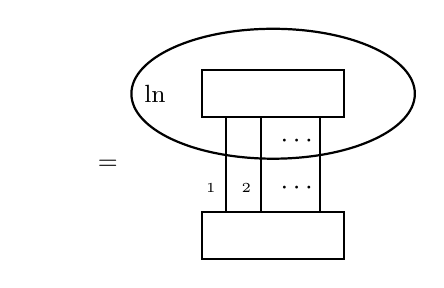
\begin{tikzpicture}[scale=0.3,thick] % , baseline = -3.5pt

\node[anchor=center] (text) at (-8,-5) {\small $\sentropyof{\probtensor}$};

\node[anchor=center] (text) at (-5,-5) {\small ${=}$};

\node[anchor=center] (text) at (-3,-2) {\small $\mathrm{ln}$};
\draw (2,-2) ellipse (6 and 2.75);

\draw (-1,-1) rectangle (5,-3);
\node[anchor=center] (text) at (2,-2) {\small $\probtensor$};
\draw (-1,-7) rectangle (5,-9);
\node[anchor=center] (text) at (2,-8) {\small $\probtensor$};
\draw (0,-5)--(0,-3); 
\draw (0,-5)--(0,-7) node[midway,left] {\tiny $\atomlegindexof{1}$}; 
\draw (1.5,-5)--(1.5,-3); 
\draw (1.5,-5)--(1.5,-7) node[midway,left] {\tiny $\atomlegindexof{2}$}; 
\node[anchor=center] (text) at (3,-4) {$\cdots$};
\draw (4,-5)--(4,-3);
\node[anchor=center] (text) at (3,-6) {$\cdots$};
\draw (4,-5)--(4,-7) node[midway,right] {\tiny $\atomlegindexof{\atomorder}$}; 

%\drawatomcore{3.5}{-8}{$\probtensor$}
%\drawatomindices{3.5}{-12}	
%\draw (5.5,-9)--(5.5,-7) node[midway,right] {\tiny $\atomlegindexof{\exformula}$};

\end{tikzpicture}
    \end{center}
    where we denote a coordinatewise transform by the logarithm as an ellipsis (see \secref{sec:coordinatewiseTransforms}).
\end{definition}

We here make the convention $\lnof{0}=-\infty$ and $0\cdot\lnof{0} = 0$, to have the Shannon entropy well-defined for distributions with non-trivial support.

Among the distributions in the same tensor space, the uniform distribution maximizes the Shannon entropy
\begin{align*}
    \sentropyof{\normationof{\ones}{\shortcatvariables}} = \sum_{\catenumeratorin}\lnof{\catdimof{\catenumerator}}
\end{align*}
and the one-hot encodings to states $\shortcatindicesin$ minimize the Shannon entropy
\begin{align*}
    \sentropyof{\onehotmapofat{\shortcatindices}{\shortcatvariables}} = 0 \, .
\end{align*}
%We understand the samples of the uniform concentration as having the maximal information con

The Shannon entropy measures the information content of a distribution and is therefore a central tool for regularization in statistical learning (see for an introduction Chapter~2 in \cite{mackay_information_2003}).
We therefore exploit this information content as a regularizer to identify a distribution among those coinciding in the answer to a collection of expectation queries.
To be more precise, let there be for $\selindexin$ query tensors $\exfunction^{\selindex}$ (see \defref{def:queries}) and $\empdistribution$ an empirical distribution.
The problem of maximal entropy with respect to coinciding expectation queries with $\empdistribution$ is then posed as
\begin{align*}
    \argmax_{\probtensor\in\bmrealprobof{\ones}} \sentropyof{\probtensor} \quad \text{subject to} \quad \uniquantwrtof{\selindexin}{\contraction{\probtensor,\exfunction^{\selindex}} = \contraction{\empdistribution,\exfunction^{\selindex}}}
\end{align*}
where $\bmrealprobof{\ones}$ is the set of probability distributions given a factored system.
We study instances of this maximal entropy problem later in \secref{sec:maxEntDuality}, where we show that its solution is a member of the exponential family, which statistic is build by the query tensors.
We will further provide connections between the problems of maximal entropy and maximum likelihood estimation.

While the Shannon entropy is a property of a single distribution, the cross-entropy is a straight forward generalization towards pairs of distributions.
We first introduce this quantity and then interpret the log-likelihood loss based on the cross-entropy.

\begin{definition}[Cross entropy and Kullback Leibler divergence]
    \label{def:crossEntropy}
    The cross-entropy between two distributions $\probwith$ and $\secprobat{\shortcatvariables}$ defined with respect to the same factored system is the quantity
    \begin{align*}
        \centropyof{\probtensor}{\secprobtensor}
        = \sum_{\catindices}  \probat{\indexedcatvariables} \cdot \left(-\lnof{\secprobtensor[\indexedshortcatvariables]}\right)
        = \sbcontraction{\probtensor,-\lnof{\secprobtensor}} \, .
    \end{align*}
    The cross-entropy is captured by the tensor network diagram
    \begin{center}
        \input{PartI/tikz_pics/probability_reasoning/cross_entropy.tex}
    \end{center}
    The Kullback-Leiber divergence between $\probwith$ and $\secprobat{\shortcatvariables}$ is the quantity
    \begin{align*}
        \kldivof{\probtensor}{\secprobtensor} = \centropyof{\probtensor}{\secprobtensor} - \sentropyof{\probtensor}  \, .
    \end{align*}
\end{definition}

%% Vanishing coordinates case
Let us notice, that we have $\centropyof{\probtensor}{\secprobtensor} = \infty$ if and only if there is a state $\shortcatindicesin$ such that $\probat{\indexedshortcatvariables}>0$ and $\secprobtensor[\indexedshortcatvariables]=0$.

% KL Divergence
The Gibbs inequality (for a proof see for example Chapter~2 in \cite{cover_elements_2006}) states that for any distributions $\probwith$ and $\secprobat{\shortcatvariables}$ we have
\begin{align*}
    \centropyof{\probtensor}{\secprobtensor} \geq \sentropyof{\probtensor} \, ,
\end{align*}
where equality holds if any only if $\probtensor=\secprobtensor$
This ensures, that the Kullback-Leiber Divergence between any distributions is positive and vanishes if and only if both distributions coincide.

We in the next lemma provide an entropic interpretation of maximum likehlihood estimation as defined in \defref{def:loss}.

\begin{lemma}
    \label{lem:centropyMLE}
    The maximum likelihood estimation \probref{prob:parameterMaxLikelihood} is equivalent to the minimization of cross-entropy and Kullback-Leibler divergence, that is
    \begin{align*}
        \argmin_{\probtensorin} \lossof{\probtensor}
        = \argmin_{\probtensorin} \centropyof{\empdistribution}{\probtensor}
        = \argmin_{\probtensorin} \kldivof{\empdistribution}{\probtensor} \, .
    \end{align*}
\end{lemma}
\begin{proof}
    Comparing the log-likelihood loss in \defref{def:loss} with the cross-entropy in \defref{def:crossEntropy}, we get
    \begin{align*}
        \lossof{\probtensor} = \centropyof{\empdistribution}{\probtensor} \,
    \end{align*}
    which established the equivalence of maximum likelihood estimation and cross-entropy minimization.
    Futher, since
    \begin{align*}
        \kldivof{\empdistribution}{\probtensor} = \centropyof{\empdistribution}{\probtensor} - \sentropyof{\empdistribution}
    \end{align*}
    and $\sentropyof{\empdistribution}$ is a constant offset in the objective, maximum likelihood estimation is equivalent to the minimization of the Kullback-Leibler divergence.
\end{proof}

% M-projection
More general than Maximum Likelihood Estimation, we define the moment projection of an arbitrary distribution $\gendistribution$ onto a set $\Gamma$ of probability distributions as the problem
\begin{align}
    \tag{$\probtagtypeinst{\mathrm{M}}{\Gamma,\gendistribution}$}\label{prob:mProjection}
    \argmax_{\probtensorin} \centropyof{\gendistribution}{\probtensor} \, .
\end{align}
With \lemref{lem:centropyMLE} we have established, that maximum likelihood estimation is the moment projection of the empirical distribution onto a set $\Gamma$.

% I-projection
We further define the information projection an arbitrary distribution $\gendistribution$ onto a set $\Gamma$ of probability distributions as the problem
\begin{align}
    \tag{$\probtagtypeinst{\mathrm{I}}{\Gamma,\gendistribution}$}\label{prob:iProjection}
    \argmax_{\probtensorin} \centropyof{\probtensor}{\gendistribution} \, .
\end{align}
The cross-entropy is not symmetric, thus the information and the moment projections do not coincide in general.
The differences of both are discussed in Chapter~8 in \cite{koller_probabilistic_2009}.

\begin{example}[Cross entropy with respect to exponential families]
    \label{exa:cEntropyExp}
    If $\secprobtensor$ is a member of an exponential family, we have %with the representation from \lemref{lem:energyCumulantRepresentation}
    \begin{align*}
        \centropyof{\probtensor}{\expdist}
        = \sbcontraction{\probtensor,\lnof{\expdist}}
        = \sbcontraction{\probtensor,\sencsstat,\canparam} - \cumfunctionof{\canparam} + \contraction{\probtensor,\lnof{\basemeasure}} \, .
    \end{align*}
    The last term vanishes, given the convention $0\cdot\lnof{0}=0$, if and only if for any $\shortcatindices$ with $\basemeasureat{\indexedshortcatvariables}=0$ we have $\probat{\indexedshortcatvariables}=0$, and is infinite instead.
    Therefore, the cross entropy between a distribution and a member of an exponential family is finite, if and only if the distribution is representable with respect to the base measure $\basemeasure$ (see \defref{def:representationBaseMeasure}).
    If $\probtensor$ is representable with respect to $\basemeasure$, we can abbreviate the cross-entropy to
    \begin{align*}
        \centropyof{\probtensor}{\expdist}
        = \contraction{\probtensor,\expenergy} -\cumfunctionof{\canparam} \, .
    \end{align*}
\end{example}



\sect{Variational Inference in Exponential Families}



\subsect{Forward and Backward Mappings}

While defined for arbitrary distributions (see \defref{def:meanPolytope}), we now consider mean parameters to members of exponential families.
First of all, they provide an alternative parameterization to the canonical parameter $\canparam$.
The computation of the mean parameter to a given canonical parameter and vice versa are the central inference problems in exponential families.
We first formalize these inference problems by the forward and backward mapping and then provide in this section further insights into these mappings.

\begin{definition}
    \label{def:meanForwardBackward}
    Let $\sstat$ be a statistic and $\basemeasure$ a base measure and consider the exponential family $\genexpfamily$
    The map
    \begin{align*}
        \forwardmap : \parspace\rightarrow\genmeanset\subset\parspace
        \defspace \forwardmapof{\canparam} = \contractionof{\expdistwith,\sencsstatwith}{\selvariable}
    \end{align*}
    is called the forward map of the exponential family and inverse, that is a map
    \begin{align*}
        \backwardmap : \imageof{\forwardmap} \subset\parspace\rightarrow \parspace
    \end{align*}
    with $\expdistof{(\sstat,\backwardmapof{\forwardmapof{\canparam}},\basemeasure)} = \expdist$ for any $\canparamwithin$, a backward map of the exponential family.
\end{definition}

% Domain of \forwardmap
We notice, that the domain of $\forwardmap$ is always $\parspace$, since the coordinates of $\forwardmapof{\canparam}$ are for any $\canparam\in\parspace$ summations over finitely many products.

%
We already know by \theref{the:meanPolytopeInteriorCharacterization}, that distributions representable by $\basemeasure$ have mean parameters in the interior of $\genmeanset$.
We now state that the elements of the corresponding exponential family $\expfamily$, which are by construction representable by $\basemeasure$, are expressive enough to reproduce the whole interior of $\genmeanset$.

\begin{theorem}
    \label{the:meanPolytopeInterior}
    For any exponential family $\genexpfamily$ the image of the forward mapping is the mean polytope except its proper faces, that is
    \begin{align*}
        \imageof{\forwardmap} = \genmeanset / \bigcup_{\genfaceset\neq\genmeanset} \genfaceset \, .
    \end{align*}
    If $\sstat$ is minimal with respect to $\basemeasure$, then $\imageof{\forwardmap}=\sbinteriorof{\genmeanset}$, the forward mapping is a bijection and the unique backward mapping its inverse.
\end{theorem}
\begin{proof}
    In case of minimal statistics, we refer for the proof of this statement to Theorem~3.3 in \cite{wainwright_graphical_2008}.
    If $\sstat$ is not minimal, we find a subset $\secsstat$ of its features such that $\secsstat$ is minimal with respect to $\basemeasure$ and there is a matrix $\matrixat{\selvariable,\secselvariable}$ such that for any distribution
    \begin{align*}
        \contractionof{\probat{\shortcatvariables},\sencodingofat{\secsstat}{\shortcatvariables,\secselvariable},\matrixat{\selvariable,\secselvariable}}{\selvariable}
        = \contractionof{\probat{\shortcatvariables},\sencodingofat{\sstat}{\shortcatvariables,\selvariable}}{\selvariable} \, .
    \end{align*}
    This subset $\secsstat$ can be found by iteratively identifying $\vectorat{\selvariable}$ and $\lambda$ such that the condition in \defref{def:minimalStatistics} is violated, and dropping a feature $\sstatcoordinateof{\selindex}$ with $\vectorat{\indexedselvariable}\neq0$.
    At each manipulation step the expressivity of the exponential family stays constant and thus $\expfamilyof{\secsstat,\basemeasure}=\expfamilyof{\sstat,\basemeasure}$.
    The matrix $\matrixat{\selvariable,\secselvariable}$ can be constructed based on the linear dependencies of the dropped features on the remaining.
    The procedure terminates, when there is no pair $\vectorat{\selvariable},\lambda$, which is equal to $\secsstat$ being minimal with respect to $\basemeasure$.
%    \begin{align*}
%        \sencodingofat{\sstat}{\shortcatvariables,\selvariable}
%        = \contractionof{\sencodingofat{\secsstat}{\shortcatvariables,\secselvariable},\matrixat{\selvariable,\secselvariable}}{\shortcatvariables,\selvariable} \, .
%    \end{align*}
    We then have %$\expfamilyof{\secsstat,\basemeasure}=\expfamilyof{\sstat,\basemeasure}$ and
    \begin{align*}
        \meansetof{\sstat,\basemeasure} / \bigcup_{\genfaceset\neq\genmeanset} \genfaceset
        = \{\contractionof{\meanparamat{\secselvariable},\matrixat{\selvariable,\secselvariable}}{\selvariable}\wcols\meanparamat{\secselvariable}\in\sbinteriorof{\meansetof{\secsstat,\basemeasure}}\} \, .
    \end{align*}
    and using that $\secsstat$ is minimal we get
    \begin{align*}
        \imageof{\forwardmap} = \genmeanset / \bigcup_{\genfaceset\neq\genmeanset} \genfaceset \, .
    \end{align*}
%    For any $\canparam$
\end{proof}

%\begin{theorem}
%    \label{the:meanPolytopeInterior}
%    For any exponential family $\genexpfamily$, where $\sstat$ is minimal with respect to $\basemeasure$, the forward mapping is a bijection of $\parspace$ and $\sbinteriorof{\genmeanset}$.
%    There is thus a unique backward mapping by the inverse of the forward mapping.
%\end{theorem}


Forward and backward maps in an exponential family $\expfamily$ are the central classes of inference, which transform the description of a member by a canonical parameter into mean parameters and vise versa.
Forward maps calculate to a canonical parameter $\canparamwith$ the corresponding mean parameter $\meanparamwith$.
For any $\canparamwith$ we have a closed form representation of this expectation query by the moment matching condition
\begin{align*}
    \meanparamwith = \contractionof{\sencsstatwith,\expdistwith}{\selvariable} \, .
\end{align*}
The forward map is thus a collection of expectation queries (see \defref{def:queries}) to compute the coordinates of the mean parameter.
The query $\sstatcoordinateof{\selindex}$ asked against $\expdistwith$ computes the coordinate $\meanparamat{\indexedselvariable}$.
%\begin{align*}
%    \forwardmapof{\canparam}
%    = \contractionof{\sencodingof{\sstat},\normationof{\basemeasure,\expof{\contraction{\sencodingof{\sstat},\canparam}}}{\shortcatvariables}}{\selvariable} \, .
%\end{align*}
% Infeasibility and turn to variational alternatives with selection encodings.
The contraction by the moment matching condition can, however, be infeasible, since it requires the instantiation of the probability distribution, which can be done by relational encodings of the statistic.
We in this section provide alternative characterization of the forward map and approximations of it, which can be computed based on the selection encoding instead.
Following \cite{wainwright_graphical_2008}, we can characterize the forward mapping to exponential families as a variational problem and provide an alternative characterization to this contraction.


\subsect{Variational Formulation}

We now formulate the forward and backward inference problems in exponential families as convex optimization problems.

The conjugate dual of the cumulative function is
\begin{align*}
    \dualcumfunction(\meanparam) = \max_{\canparam\in\parspace} \contraction{\meanparam,\canparam} - \cumfunctionof{\canparam} \, .
\end{align*}

\begin{lemma}\label{lem:gradientCumfunction}
    Let $\canparam\in\parspace$ and $\meanparamwith$ the corresponding mean parameter.
    For the gradient of $\cumfunction$ evaluated at $\canparam$ we have
    \begin{align*}
        \gradwrtat{\seccanparamat{\selvariable}}{\canparam} \cumfunctionof{\seccanparam} = \meanparamat{\selvariable}
    \end{align*}
    If the statistic $\sstat$ is minimal with respect to $\basemeasure$, then also
    \begin{align*}
        \gradwrtat{\secmeanparamat{\selvariable}}{\meanparam} \dualcumfunctionof{\secmeanparam}
        = \canparamat{\selvariable} \, .
    \end{align*}
\end{lemma}
\begin{proof}
    We have
    \begin{align*}
        \gradwrtat{\canparam}{\seccanparam} \cumfunctionof{\seccanparam} \\
        & = \gradwrtat{\canparam}{\seccanparam} \lnof{\contraction{\expof{\contractionof{\sencsstatwith,\canparamwith}{\shortcatvariables}},\basemeasure}} \\
        & = \frac{1}{\contraction{\expof{\contractionof{\sencsstatwith,\canparamwith}{\shortcatvariables}}}}  \cdot \contractionof{\sencsstatwith,\expof{\contractionof{\sencsstatwith,\canparamwith}{\shortcatvariables}},\basemeasure}{\selvariable}\\
        & = \contractionof{\expdistwith,\sencsstatwith}{\selvariable} \, .
    \end{align*}
    For the proof of the second claim we refer to Appendix B.2 in \cite{wainwright_graphical_2008}.
\end{proof}

\begin{theorem}[Variational backward map]
    For any $\meanparam\in\interiorof{\meanset}$ choose
    \begin{align*}
        \canparamat{\selvariable} \in \argmax_{\canparam} \contraction{\meanparam,\canparam} - \cumfunctionof{\canparam} \, .
    \end{align*}
    Then $\meanparam$ is the mean parameter to $\expdist$.
\end{theorem}
\begin{proof}
    The maximization over $\canparam$ is an unconstrained concave maximization problem and the optimum is characterized by
    \begin{align*}
        0 = \gradwrtat{\canparam}{\seccanparam}\left(\contraction{\meanparam,\canparam} - \cumfunctionof{\canparam}\right)
    \end{align*}
    which reads
    \begin{align*}
        \meanparamat{\selvariable} = \gradwrtat{\canparam}{\seccanparam[\selvariable]} \cumfunctionof{\canparam} \, .
    \end{align*}
    With \lemref{lem:gradientCumfunction}, the gradient vanishes if and only if $\meanparam$ is the mean parameter to $\expdist$.
\end{proof}

The backward map is closely connected with the conjugate dual of $\cumfunction$.
In particular, while the conjugate dual is defined by the maximization problem
\begin{align*}
    \dualcumfunctionof{\meanparam} = \max_{\canparam\in\parspace} \contraction{\meanparam,\canparam} - \cumfunctionof{\canparam}
\end{align*}
the backward map returns the position of the maximum in $\parspace$.

\begin{lemma}\label{lem:dualCumEntropy}
    For any $\canparam$ with mean parameter $\meanparam$ we have
    \begin{align*}
        \dualcumfunction(\meanparam) = - \sentropyof{\expdist} \, .
    \end{align*}
\end{lemma}
\begin{proof}
    We have
    \begin{align*}
        \canparam \in \argmax_{\canparam} \contraction{\meanparam,\canparam} - \cumfunctionof{\canparam}
    \end{align*}
    if and only if
    \begin{align*}
        \meanparamwith = \contractionof{\expdistwith,\sencsstatwith}{\selvariable} \, .
    \end{align*}
    Therefore
    \begin{align*}
        \dualcumfunction(\meanparam) = \contraction{\expdistwith,\sencsstatwith,\canparam} - \cumfunctionof{\canparam}
        = \contraction{\expdistwith, \lnof{\expdistwith}}
        = - \sentropyof{\expdist} \, .
    \end{align*}
\end{proof}

We can use this insight to provide a variational characterization of the forward mapping.

\begin{theorem}[Variational forward mapping]
    Let $\sstat$ be a minimal statistic with respect to $\basemeasure$.
    Given $\canparam$, there is a unique $\meanparam$ with
    \begin{align*}
         \meanparam \in \argmax_{\meanparam\in\meanset} \contraction{\meanparam,\canparam} + \sentropyof{\expdistof{\sstat,\meanparam,\basemeasure}} %-  \dualcumfunction(\meanparam)
    \end{align*}
    and $\meanparam$ is the mean parameter to $\expdistwith$.
    Here, we denote by $\expdistof{\sstat,\meanparam,\basemeasure}$ the member of the exponential family with the mean parameter $\meanparam$.
\end{theorem}
\begin{proof}
    By strong duality, we have $\left(\cumfunction\right)^{**}=\cumfunction$ and
    \begin{align*}
        \cumfunction(\canparam) = \max_{\meanparam\in\meanset} \contraction{\meanparam,\canparam} -  \dualcumfunction(\meanparam) \, .
    \end{align*}
    The statement then follows from the first order condition, where we use the gradient \lemref{lem:gradientCumfunction}, and the characterization of $\dualcumfunction$ by \lemref{lem:dualCumEntropy}. % Do we need to assume minimal statistics?
\end{proof}

%We have at any $\canparam\in\parspace$
%\begin{align*}
%    \gradwrtat{\canparam}{\seccanparam} \cumfunctionof{\seccanparam} = \meanparamat{\selvariable}
%\end{align*}
%and thus
%\begin{align*}
%    \meanparamat{\selvariable} = \argmax_{\meanparam\in\meanset}
%\end{align*}


\sect{Maximum entropy distributions}

\red{We characterize in this section to any mean parameter the reproducing distribution with maximum entropy, and investigate their modes and tensor network representation.
As we will show, the distributions with maximal entropy are in exponential families with base measure determined by the smallest face, which contains the mean parameter.
}

% To expectation queries, as an example!
The mean parameters are computed as collections of expectation queries to $\sstatcoordinateof{\selindex}$, which are answered against distributions in $\bmrealprobof{\basemeasure}$.
For any $\selindexin$ we have for the mean parameter $\meanparamwith$ reproduced by a distribution $\probwith$
\begin{align*}
    \meanparamat{\indexedselvariable}
    = \expectationof{\sstatcoordinateof{\selindex}}
    = \contraction{\sencsstatat{\shortcatvariables,\indexedselvariable},\probwith} \, .
\end{align*}


\subsect{Entropy maximization problem}\label{sec:maxEntDuality}


The entropy maximization problem with respect to matching expected statistics $\genmean\in\genmeanset$ is the optimization problem
\begin{align}
    \tag{$\probtagtypeinst{\entropysymbol}{\sstat,\basemeasure,\genmean}$}\label{prob:maxEntropy} % Notation clash with cross-entropy!
    \argmax_{\probtensor\in\bmrealprobof{\basemeasure}} \sentropyof{\probtensor} \quad \text{subject to} \quad
    \sbcontractionof{\probtensor,\sencsstat}{\selvariable} = \genmeanat{\selvariable}
\end{align}
where by $\bmrealprobof{\basemeasure}$ we denote all distributions, which are representable with respect to a base measure $\basemeasure$.

% Feasibility
By definition of the mean polytope, \probref{prob:maxEntropy} has a feasible distribution if and only if $\genmeanat{\selvariable}\in\genmeanset$.
If this condition holds, we now characterize the solution of \probref{prob:maxEntropy}.
First of all, we show that the maximum entropy distribution is in the exponential family $\genexpfamily$, when $\meanparam$ does not lie on a proper face of $\genmeanset$.
We then drop this assumption and generalize the statement to exponential families with refined base measures.

\begin{theorem}\label{the:maxEntropyInterior}
    If the only face $\genfacesetof{\facecondset}$ of $\genmeanset$ with $\meanparam\in\genfacesetof{\facecondset}$ is $\genmeanset$ itself, then the solution of the maximum entropy distribution is the unique distribution
    \begin{align*}
        \expdistofat{\sstat,\meanparam,\basemeasure}{\shortcatvariables}\in\expfamilyof{\sstat,\basemeasure}
    \end{align*}
    with $\contractionof{\expdistofat{\sstat,\meanparam,\basemeasure}{\shortcatvariables},\sencsstatwith}{\selvariable}=\meanparamat{\selvariable}$.
\end{theorem}
\begin{proof}
    By \theref{the:meanPolytopeInterior}, since by assumption
    \begin{align*}
        \meanparamwith \in \genmeanset / \bigcup_{\genfaceset\neq\genmeanset} \genfaceset \, ,
    \end{align*}
    there is a canonical parameter $\canparam$ with
    \begin{align*}
        \contractionof{\expdistofat{\sstat,\canparam,\basemeasure}{\shortcatvariables},\sencsstatwith}{\selvariable}=\meanparamat{\selvariable}
    \end{align*}

    For any other feasible distribution $\secprobat{\shortcatvariables}$ we also have $\contractionof{\secprobat{\shortcatvariables},\sencsstatwith}{\selvariable}=\meanparamat{\selvariable}$ and thus
    \begin{align*}
        \centropyof{\secprobtensor}{\expdistof{(\sstat,\canparam,\basemeasure)}}
        &= -\contraction{\secprobtensor,\lnof{\expdistofat{(\sstat,\canparam,\basemeasure)}{\shortcatvariables}}} \\
        &= -\contraction{\secprobtensor,\contractionof{\sencsstatwith,\canparamwith}{\shortcatvariables}} + \cumfunctionof{\canparam} \\
        &= - \contraction{\canparam,\meanparam} + \cumfunctionof{\canparam} \\
        &= \sentropyof{\expdistof{(\sstat,\canparam,\basemeasure)}} \, .
    \end{align*}

    With the Gibbs inequality we have if $\secprobtensor\neq\expdistof{(\sstat,\canparam,\basemeasure)}$
    \begin{align*}
        \sentropyof{\expdistof{(\sstat,\estcanparam,\basemeasure)}} - \sentropyof{\secprobtensor}
        = \centropyof{\secprobtensor}{\expdistof{(\sstat,\estcanparam,\basemeasure)}} - \sentropyof{\secprobtensor} > 0 \, .
    \end{align*}

    Therefore, if $\secprobtensor$ does not coincide with$\expdistof{(\sstat,\estcanparam,\basemeasure)}$, it is not a solution of \probref{prob:maxEntropy}.
\end{proof}


%\begin{theorem}
%    \label{the:maxEntInterior}
%    Let $\sstat$ be a minimal statistic with respect to a base measure $\basemeasure$.
%    For any $\genmean\in\sbinteriorof{\genmeanset}$ the solution of \probref{prob:maxEntropy} is the distribution $\expdistof{(\secsstat,\estcanparam,\secbasemeasure)}$, where $\estcanparam=\backwardmapwrtof{\secsstat,\secbasemeasure}{\secmeanparam}$.
%\end{theorem}
%\begin{proof}
%    Since $\genmean\in\sbinteriorof{\genmeanset}$, \theref{the:meanPolytopeInteriorCharacterization} implies the existence of $\estcanparam$ such that
%    \[ \genmeanat{\selvariable} = \sbcontractionof{\expdistof{(\sstat,\estcanparam,\basemeasure)},\sencsstat}{\selvariable}   \, . \]
%    We now follow the argumentation of the proof of Theorem~20.2 in \cite{koller_probabilistic_2009}.
%    Let $\secprobtensor$ further be an arbitrary distribution, possibly different from $\expdistof{(\sstat,\estcanparam,\basemeasure)}$, such that
%    \[ \genmeanat{\selvariable} = \sbcontractionof{\secprobtensor,\sencsstat}{\selvariable}  \, . \]
%    We then have
%    \begin{align*}
%        \sentropyof{\expdistof{(\sstat,\estcanparam,\basemeasure)}}
%        = \centropyof{\secprobtensor}{\expdistof{(\sstat,\estcanparam,\basemeasure)}}
%    \end{align*}
%
%    With the Gibbs inequality we have if $\secprobtensor\neq\expdistof{(\sstat,\estcanparam,\basemeasure)}$
%    \begin{align*}
%        \sentropyof{\expdistof{(\sstat,\estcanparam,\basemeasure)}} - \sentropyof{\secprobtensor}
%        = \centropyof{\secprobtensor}{\expdistof{(\sstat,\estcanparam,\basemeasure)}} - \sentropyof{\secprobtensor} > 0 \, .
%    \end{align*}
%
%    Therefore, if $\secprobtensor$ does not coincide with$\expdistof{(\sstat,\estcanparam,\basemeasure)}$, it is not a solution of Problem~\ref{prob:maxEntropy}.
%    %Classical result based on duality of maximum entropy and maximum likelihood, shown e.g. in Koller Book.
%\end{proof}

% Interpretation
Let us highlight the fact, that in \probref{prob:maxEntropy} we did not restrict to distributions in an exponential family and only demanded representability with respect to the base measure.
When choosing the trivial base measure, this does not pose a restriction on the distributions.
\theref{the:maxEntInterior} states, that when the maximum entropy problem has a solution (i.e. $\genmean\in\genmeanset$), then the solution is in the exponential family to the statistic $\sstat$.

% Generalization
When $\genmean\notin\sbinteriorof{\genmeanset}$, the mean paramater is by \theref{the:meanPolytopeInteriorCharacterization} not reproducable by a member of the exponential family $\expfamilyof{\sstat,\basemeasure}$.
Instead, in combination with the base measure refinement \algoref{alg:baseMeasureRefinement}, we show that the solution is in a refined exponential family.
% dropping the assumption that the mean parameters are in the interior of the mean parameter polytope.

\begin{theorem}\label{the:maxEntropyFace}
    Let $\genfacesetof{\facecondset}$ be the minimal face of $\genmeanset$ such that $\meanparamat{\selvariable}\in\genfacesetof{\facecondset}$.
    Then, the solution of the maximum entropy problem is the distribution
    \begin{align*}
        \expdistof{\sstat,\meanparam,\secbasemeasure}
    \end{align*}
    where the base measure $\secbasemeasure$ is the refinement of $\basemeasure$ by the face measure $\genfacemeasure$, that is
    \begin{align*}
        \secbasemeasureat{\shortcatvariables} = \contractionof{\basemeasureat{\shortcatvariables},\genfacemeasureat{\shortcatvariables}}{\shortcatvariables} \, .
    \end{align*}
\end{theorem}
\begin{proof}
    By \theref{the:facePolytopeCharacterization} all feasible distributions for the maximum entropy problem have to be representable by the face measure $\genfacemeasure$.
    Since the feasible distributions are further restricted to those representable by $\basemeasure$, they are also representable by the refined base measure $\secbasemeasure$.
    Now, by \theref{the:faceAsRefinedPolytope} the face itself is a polytope $\meansetof{\sstat,\secbasemeasure}$ and the smallest face containing $\meanparam$ is the polytope itself.
    We thus arrive at the claim by applying \theref{the:maxEntropyInterior} on the polytope $\meansetof{\sstat,\secbasemeasure}$.
\end{proof}


%\begin{theorem}
%    \label{the:maxEntMaxLikeDuality}
%    Let $\sstat$ be a statistic and $\basemeasure$ a base measure.
%    For any $\genmean\in\genmeanset$, let $\secsstat,\secbasemeasure$ and $\secmeanparam$ be the outputs of \algoref{alg:baseMeasureRefinement} when passing $\sstat,\basemeasure$ and $\genmean$ as input.
%    Then, the distribution $\expdistof{(\secsstat,\estcanparam,\secbasemeasure)}$, where $\estcanparam=\backwardmapwrtof{\secsstat,\secbasemeasure}{\secmeanparam}$, solves \probref{prob:maxEntropy}.
%\end{theorem}
%\begin{proof}
%    By \theref{the:baseMeasureRefinement}, a distribution $\probtensor$ is feasible for the problem \probref{prob:maxEntropy} if and only if
%    \begin{align*}
%        \contractionof{\probwith,\sencodingofat{\secsstat}{\shortcatvariables,\secselvariable}} = \secmeanparam[\secselvariable] \, .
%    \end{align*}
%    Therefore, a distribution solves the maximum entropy problem for $\sstat$ and $\meanparam$, if and only if it solves the maximum entropy problem for $\secsstat$ and $\secmeanparam$.
%    Since \theref{the:baseMeasureRefinement} further ensures, that $\secmeanparam\in\sbinteriorof{\meansetof{\secsstat,\secbasemeasure}}$, the claim follows from \theref{the:maxEntInterior}.
%%    \theref{the:baseMeasureRefinement} and the above Lemma.
%\end{proof}

% Minimality of the refined base measure
\theref{the:maxEntropy} implies, that the by the face measure refined base measure $\secbasemeasure$ is minimal for the maximum entropy problem, in the sense that the solving distribution is positive with respect to it and all feasible distributions have to be representable by it.
This highlights the fact, that the maximum entropy distribution does not vanish beyond those states, which are necessary to vanish to lie on the respective face. %by \theref{the:baseMeasureRefinement}.


\subsect{Tensor Network Representation}

% Representation
Maximum entropy distributions with respect to constraints $\meanparamat{\selvariable}=\contractionof{\probtensor,\sencsstat}{\selvariable}$ always have the sufficient statistic $\sstat$.
They are represented in $\hlnsetof{\sstat}$, if and only if the face measure of any face $\facecondset$ such that
\begin{align*}
    \meanparamat{\selvariable} \in \genfaceset{\facecondset}
\end{align*}
is in $\hlnsetof{\sstat}$.
This is for example the case when $\meanparamat{\selvariable}\in\sbinteriorof{\genmeanset}$.
In general, we find a $\cpformat$ decomposition as sketched in \figref{fig:maxEntropyActcore}.

\begin{figure}
    \begin{center}
        \begin{tikzpicture}[scale=0.4,thick,xscale=1] % , baseline = -3.5pt

    \begin{scope}[shift={(-15,0)}]
        \draw (-1,-1) rectangle (5,-3);
        \node[anchor=center] (text) at (2,-2) {\small $\probtensor$};
        \draw[->-] (0,-3)--(0,-5) node[midway,left] {\tiny $\catvariableof{0}$};
        \draw[->-] (1.5,-3)--(1.5,-5) node[midway,left] {\tiny $\catvariableof{1}$};
        \node[anchor=center] (text) at (3,-4) {$\cdots$};
        \draw[->-] (4,-3)--(4,-5) node[midway,right] {\tiny $\catvariableof{\atomorder\shortminus1}$};

        \node[anchor=center] (text) at (8,-2) {$= \,\frac{1}{\partitionfunction} \cdot $};
    \end{scope}

    %% Condition cores: Boolean cores selecting faces
    \draw[\concolor] (4,3) to[bend right=20] (2,5);
    \draw[\concolor] (0,3) to[bend left=20] (2,5);
    \draw[fill,\concolor] (2,5) circle (\dotsize);

    \draw[\concolor] (-1,1) rectangle (1,3);
    \node[anchor=center,\concolor] (text) at (0,2) {$\conactcoreof{{0}}$};

    \draw[\concolor] (3,1) rectangle (5,3);
    \node[anchor=center,\concolor] (text) at (4,2) {$\conactcoreof{{\seccatorder\shortminus1}}$};

    \draw[->-] (0,-1)--(0,0);
    \node[right] (text) at (0,0) {\tiny $\headvariableof{0}$};
    \draw[\concolor] (0,0)--(0,1);
    \drawvariabledot{0}{0}
    \node[anchor=center] (text) at (2,0) {$\cdots$};

    \draw[\probcolor] (0,0) -- (-2,0);
    \draw[\probcolor] (-2,1) rectangle (-4,-1);
    \node[anchor=center,\probcolor] (text) at (-3,0) {$\actcoreof{0}$};

    \draw[->-] (4,-1)--(4,0);
    \node[left] (text) at (4,0) {\tiny $\headvariableof{\seccatorder\shortminus1}$};
    \draw[\concolor] (4,0)--(4,1);
    \drawvariabledot{4}{0}

    \draw[\probcolor] (4,0) -- (6,0);
    \draw[\probcolor] (6,1) rectangle (8,-1);
    \node[anchor=center,\probcolor] (text) at (7,0) {$\actcoreof{\seccatorder\shortminus1}$};

    \draw (-1,-1) rectangle (5,-3);
    \node[anchor=center] (text) at (2,-2) {\small $\rencodingof{\sstat}$};
    \draw[-<-] (0,-3)--(0,-5) node[midway,left] {\tiny $\catvariableof{0}$};
    \draw[-<-] (1.5,-3)--(1.5,-5) node[midway,left] {\tiny $\catvariableof{1}$};
    \node[anchor=center] (text) at (3,-4) {$\cdots$};
    \draw[-<-] (4,-3)--(4,-5) node[midway,right] {\tiny $\catvariableof{\atomorder\shortminus1}$};

    \draw (-1,-1) rectangle (5,-3);
    \node[anchor=center] (text) at (2,-2) {\small $\rencodingof{\sstat}$};
    \draw[-<-] (0,-3)--(0,-5) node[midway,left] {\tiny $\catvariableof{0}$};
    \draw[-<-] (1.5,-3)--(1.5,-5) node[midway,left] {\tiny $\catvariableof{1}$};
    \node[anchor=center] (text) at (3,-4) {$\cdots$};
    \draw[-<-] (4,-3)--(4,-5) node[midway,right] {\tiny $\catvariableof{\atomorder\shortminus1}$};

%    \node[anchor=center] (text) at (6,-4.5) {$.$};

%\drawatomcore{3.5}{-8}{$\probtensor$}
%\drawatomindices{3.5}{-12}	
%\draw (5.5,-9)--(5.5,-7) node[midway,right] {\tiny $\catvariableof{\exformula}$};

\end{tikzpicture}
    \end{center}
    \caption{
        Tensor network decomposition of maximum entropy distributions to the constraint $\meanparamat{\selvariable}=\contractionof{\probtensor,\sencsstat}{\selvariable}$.
        Blue: Constraint activation cores $\conactcoreof{\selindex}$ in an $\cpformat$ decomposition, representing the face measure to the minimal face, such that $\meanparam\in\genfacesetof{\facecondset}$.
        Red: Probabilistic activation cores $\actcoreof{\selindex}$ in an elementary decomposition, where each leg core is a scaled exponentials evaluated on the enumerated image $\imageof{\sstatcoordinateof{\selindex}}$.
    }\label{fig:maxEntropyActcore}
\end{figure}



\subsect{Modes of maximum entropy distributions}

\begin{figure}[t!]
    \begin{center}
        \input{PartI/tikz_pics/probability_reasoning/meanset_sketch_face.tex}
    \end{center}
    \caption{Sketch of a face $\genfacesetof{\canparam}$ to the normal $\canparamwith$.
    The face is characterized by those mean parameters in $\genmeanset$, which maximize the contraction with $\canparamwith$.
    The sketched distance of the origin $\zerosat{\canparam}$ of $\rr^{\seldim}$ to the affine hull of the face is further related to the maximal contraction.
    }\label{fig:meansetSketchFace}
\end{figure}

\red{We now show, that the face base measures coincide with the solutions of mode queries.
Motivated by this fact, we define max cones of canonical parameters, which parametrized distributions coincide in their modes.}

%% To Reasoning: Characterization of faces by maxima
Let us now investigate, that faces of $\genmeanset$ are the solutions of linear optimization problems constrained by $\genmeanset$ (see \figref{fig:meansetSketchFace}).
Since such solution sets are intersections of the boundary of $\genmeanset$ with half-spaces, they are faces.
In the next theorem we show, how linear optimization problems are constructed to match a given face.

%which is build by faces, we
%Let us now connect faces with the solutions of maximization problems.

\begin{theorem}
    \label{the:faceNormal}
    For any non-empty face $\genfacesetof{\facecondset}$ to a subset $\mathcal{I}\subset[n]$ there is a vector $\canparamwith$, which we call a normal of the face, such that
    \begin{align*}
        \genfacesetof{\facecondset} = \cangenmeansetargmax  \, .
    \end{align*}
    For any collection of positive $\lambda_i$, where $i\in\facecondset$, the vector
    \begin{align*}
        \canparamwith = \sum_{i\in\facecondset} \lambda_i\cdot\normalvecofat{i}{\selvariable}
    \end{align*}
    is a normal for $\genfacesetof{\facecondset}$.
    %% UNCLEAR if this is true-> Are all possible normals in the span
%	If $\canparamwith$ is a normal to a face, then for any positive scalars $\lambda[\selvariable]$ also the vector
%		\[ \seccanparam\left[\selvariable\right] = \contractionof{\canparamwith,\labmda[\selvariable]}{\selvariable} \]
%	is a normal to the same face.
\end{theorem}
\begin{proof}
    The first claim follows trivially from the second.
    To show the second claim, let there be for $i\in\facecondset$ arbitrary positive scalars $\lambda_i$.
    Since the face is non-empty, there is a $\meanparamwith$ with
    \begin{align*}
        \contraction{\meanparamwith,\normalvecofat{i}{\selvariable}}=\normalboundof{i}
    \end{align*}
    for all $i\in\facecondset$.
    Since any $\meanparam\in\genmeanset$ obey
    \begin{align*}
        \contraction{\meanparamwith,\normalvecofat{i}{\selvariable}}\leq \normalboundof{i}
    \end{align*}
    it follows that
    \begin{align*}
        \max_{\meanparam\in\genmeanset} \contraction{\canparamwith,\meanparamwith}
        = \sum_{i\in\facecondset} \lambda_i \cdot \normalboundof{i} \, .
    \end{align*}
    The maximum is attained at a $\meanparamwith$, if and only if the equations $\contraction{\meanparamwith,\normalvecofat{i}{\selvariable}}=\normalboundof{i}$ are satisfied for $i\in\facecondset$.
    This is equal to $\meanparamwith\in\genfacesetof{\facecondset}$.
\end{proof}

As we show next, also a converse statement holds, namely that for any vector $\canparamwith$ we find a face $\genfacesetof{\facecondset}$, such that the $\canparamwith$ is a face normal to that face.

\begin{theorem}
    \label{the:modeQueryFaceBM}
    For any $\canparamwith$ we find a subset $\mathcal{I}\subset[n]$, such that
    \begin{align*}
        \cangenmeansetargmax = \genfacesetof{\facecondset} \, .
    \end{align*}
\end{theorem}
\begin{proof} % Not a smooth proof, improve!
    We first notice, that
    \begin{align*}
       & \cangenmeansetargmax \\
       & \quad  = \convhullof{\sencsstatat{\indexedshortcatvariables,\selvariable} \, : \, \shortcatindices\in\argmax_{\shortcatindicesin} \contraction{\canparamwith,\sstatat{\shortcatindices}}} \, .
    \end{align*}
    Further, since the contraction with $\canparamwith$ is linear, the set $\cangenmeansetargmax$ is contained in the boundary of the polytope $\genmeanset$.
    We can conlcude, that the set is a face, that is we find a subset $\mathcal{I}\subset[n]$ with
    \begin{align*}
        \genfacesetof{\facecondset} = \cangenmeansetargmax \, .
    \end{align*}
\end{proof}

% Notation
In a slide abuse of notation, we denote in this case $\genfacesetof{\canparam} = \genfacesetof{\facecondset}$.

% Mode queries
\theref{the:modeQueryFaceBM} provides a geometric perspective for mode queries.
An arbitrary tensor $\hypercorewith$ can be understood to be a canonical parameter of the exponential family with statistic $\naivestat$, and base measure $\onesat{\shortcatvariables}$.
For this exponential family, $\bmrealprobof{\ones}$ coincides with the polytope of mean parameters, and is a standard simplex.
Continuing our discussion in \secref{sec:modeQueries}, we have for any $\arbset\subset\facstates$ and $\basemeasure$ being the subset encoding of $\arbset$ that
\begin{align*}
    \max_{\shortcatindices\in\arbset} \hypercoreat{\indexedshortcatvariables} =
    \max_{\meanparamat{\shortcatvariables}\in\bmrealprobof{\basemeasure}} \contraction{\hypercoreat{\shortcatvariables},\meanparamat{\shortcatvariables}} \, .
\end{align*}
The maximum is attained exactly for the mean parameters
\begin{align*}
    \meanparamat{\shortcatvariables}\in
    \convhullof{\onehotmapofat{\shortcatindices}{\shortcatvariables} \, : \, \shortcatindices\in\argmax_{\shortcatindices\in\arbset} \hypercoreat{\indexedshortcatvariables}} \, .
\end{align*}
Answering the mode query is thus the characterization of the face of the standard simplex with face normal $\hypercorewith$.

% Decompositions of \hypercore
Let us now consider cases where the queried tensor $\hypercore$ has a tensor network decomposition.
This is the case for energy tensors to members of exponential families, for which we have a decomposition into selection encodings $\sencsstatwith$ and canonical parameters $\canparamwith$.
In most generality we assume a decomposition of $\hypercore$ by a tensor network on a hypergraph $\graph=(\nodes,\edges)$, where $[\catorder]\subset\nodes$ as
\begin{align*}
    \hypercorewith = \contractionof{\extnetasset}{\shortcatvariables} \, .
\end{align*}
Let us choose a subset $\secedges\subset\edges$ and
\begin{align*}
    \max_{\shortcatindices\in\arbset} \hypercoreat{\indexedshortcatvariables}
    = \max_{\shortcatindices\in\arbset} \contraction{\{\onehotmapofat{\shortcatindices}{\shortcatvariables}\} \cup \extnetasset}
%        = \max_{\shortcatindices\in\arbset} \contraction{\onehotmapofat{\shortcatindices}{\shortcatvariables},\hypercoreat{\indexedshortcatvariables}}
\end{align*}
We now split the contractions (see \theref{the:splittingContractions}) to contract the cores $\edges/\secedges$ with the one-hot encoding first and keeping $\secnodes=\bigcup_{\edge\in\secedges}\edge$ open.
With this we get
\begin{align*}
    & \max_{\shortcatindices\in\arbset} \hypercoreat{\indexedshortcatvariables} \\
    & = \max_{\shortcatindices\in\arbset}
    \contraction{
        \contractionof{\{\onehotmapofat{\shortcatindices}{\shortcatvariables}\} \cup \left\{\hypercoreofat{\edge}{\catvariableof{\edge}}\, : \, \edge\in\edges/\secedges\right\}}{\catvariableof{\secnodes}},
        \contractionof{\left\{\hypercoreofat{\edge}{\catvariableof{\edge}}\, : \, \edge\in\secedges\right\}}{\catvariableof{\secnodes}}
    } \, .
\end{align*}
This optimization problem is the characterization of vectors, which convex hull is the face in the polytope
\begin{align*}
    \meanset = \left\{\{\contractionof{\onehotmapofat{\shortcatindices}{\shortcatvariables}\} \cup \left\{\hypercoreofat{\edge}{\catvariableof{\edge}}\, : \, \edge\in\edges/\secedges\right\}}{\catvariableof{\secnodes}} \, : \, \shortcatindices\in\arbset \right\}
\end{align*}
with the face normal
\begin{align*}
    \canparamat{\catvariableof{\secnodes}} =
    \contractionof{\left\{\hypercoreofat{\edge}{\catvariableof{\edge}}\, : \, \edge\in\secedges\right\}}{\catvariableof{\secnodes}} \, .
\end{align*}

We define for each face the normal cone
\begin{align*}
    \maxcone = \{\canparam\wcols\canparam\in\parspace\ncond\argmax_{\meanparam\in\genmeanset}\contraction{\canparam,\meanparam}=\genfaceset\} \, .
\end{align*}

% Maybe earlier to avoid minimal statistics discussion
%\begin{definition}
%    We say, that a set $\arbset\subset\parspace$ is effectively open, if $\arbset$ is contained in an affine subspace and open in that affine subspace.
%\end{definition}

\begin{lemma}
    For each face $\facecondset$, $\maxcone$ is a convex cone. % Missing: effectively open
\end{lemma}
\begin{proof}
    $\maxcone$ is a cone, since for any $\canparam\in\maxcone$ and $\lambda>0$ we have
    \begin{align*}
        \genfaceset = \argmax_{\meanparam\in\genmeanset} \contraction{\canparam,\meanparam} = \argmax_{\meanparam\in\genmeanset} \contraction{\lambda\cdot\canparam,\meanparam} \, .
    \end{align*}

    % Convex
    $\maxcone$ is convex, since for $\canparam,\seccanparam\in\maxcone$ and $\lambda\in(0,1)$ we have
    \begin{align*}
        \genfaceset = \argmax_{\meanparam\in\genmeanset} \contraction{\canparam,\meanparam} = \argmax_{\meanparam\in\genmeanset} \contraction{\seccanparam,\meanparam} \, .
    \end{align*}
    It follows
    \begin{align*}
        \genfaceset = \argmax_{\meanparam\in\genmeanset} \contraction{\lambda\cdot\canparam+(1-\lambda)\cdot\seccanparam,\meanparam}
    \end{align*}
    and $\lambda\cdot\canparam+(1-\lambda)\cdot\seccanparam \in\maxcone$.

    % Show that Effectively open - Missing!
\end{proof}



\begin{lemma}\label{lem:faceSetsToMaxCones}
    For two non-empty faces $\facecondsetof{0}$ and $\facecondsetof{1}$ we have % Non-empty needed? Can deal with face 1 empty, but with face 0 empty?
    \begin{align*}
        \genfacesetof{\facecondsetof{0}} \subset \genfacesetof{\facecondsetof{1}}
    \end{align*}
    if and only if
    \begin{align*}
        \genmaxconeof{\facecondsetof{1}} \subset \closureof{\genmaxconeof{\facecondsetof{0}}} \, .
    \end{align*}
\end{lemma}
\begin{proof}
    \proofrightsymbol Let us assume $\genfacesetof{\facecondsetof{0}} \subset \genfacesetof{\facecondsetof{1}}$ and let us choose arbitrary $\canparamof{0}\in\genmaxconeof{\facecondsetof{0}},\,\canparamof{1}\in\genmaxconeof{\facecondsetof{1}}$.
        It suffices to show, that for all $\lambda\in(0,1)$ we have $\lambda\cdot\canparamof{0}+(1-\lambda)\cdot\canparamof{1}\in\genmaxconeof{\facecondsetof{0}}$, since this implies $\canparamof{1}\in\closureof{\genmaxconeof{\facecondsetof{0}}}$.
        By assumption we have
        \begin{align*}
            \argmax_{\meanparam\in\genmeanset} \contraction{\canparamof{0},\meanparam} \subset  \argmax_{\meanparam\in\genmeanset} \contraction{\canparamof{1},\meanparam}
        \end{align*}
        and thus
        \begin{align*}
            \argmax_{\meanparam\in\genmeanset} \contraction{\lambda\cdot\canparamof{0}+(1-\lambda)\cdot\canparamof{1},\meanparam} = \argmax_{\meanparam\in\genmeanset} \contraction{\canparamof{0},\meanparam}
        \end{align*}
        which implies $\lambda\cdot\canparamof{0}+(1-\lambda)\cdot\canparamof{1}\in\genmaxconeof{\facecondsetof{0}}$.
    \proofleftsymbol Conversely, let us assume $\genmaxconeof{\facecondsetof{1}} \subset \closureof{\genmaxconeof{\facecondsetof{0}}}$.
        We then find a sequence $\left(\canparamof{n}\right)_{n\in\nn}$ with $\canparamof{n}\in\genmaxconeof{\facecondsetof{0}}$ for $n\in\nn$ and which limit $\canparam$ exists in $\genmaxconeof{\facecondsetof{1}}$.
        For an arbitrary $\catindex\in\stateset$ with $\sstatencodingat{\catindex}\in\genfacesetof{\facecondsetof{0}}$ we have
        \begin{align*}
            \contraction{\canparam,\sstatencodingat{\catindex}}
            &= \lim_{n\rightarrow\infty} \contraction{\canparamof{n},\sstatencodingat{\catindex}} \\
            &= \lim_{n\rightarrow\infty} \max_{\seccatindex\in\stateset} \contraction{\canparamof{n},\sstatencodingat{\seccatindex}} \\
            &= \max_{\seccatindex\in\stateset} \contraction{\canparam,\sstatencodingat{\seccatindex}}
        \end{align*}
        and therefore $\sstatencodingat{\catindex}\in\genfacesetof{\facecondsetof{1}}$.
        Note, that we used in the third equation, that $\stateset$ is finite.% and thus avoided to justify these equations based on convexity. -> More precise statement needed !
        We use this property for all elements of the preimage of $\facecondsetof{0}$ and get
        \begin{align*}
            \genfacesetof{\facecondsetof{0}}
            &= \convhullof{\sstatencodingat{\catindex}\wcols\catindex\in\argmax_{\seccatindex\in\stateset}\contraction{\canparamof{1},\sstatencodingat{\seccatindex}}} \\
            &\subset \convhullof{\sstatencodingat{\catindex}\wcols\catindex\in\argmax_{\seccatindex\in\stateset}\contraction{\canparam,\sstatencodingat{\seccatindex}}} \\
            &= \genfacesetof{\facecondsetof{1}} \, .
        \end{align*}
\end{proof}

\lemref{lem:faceSetsToMaxCones} suggests that the partial order of faces by inclusion is mimiked by another partial order on the max cones, sketched in \figref{fig:max_cone_sketch}.
We now consider the set of cones with this partial order, and show that this set is homomorphic to the face lattice.

\begin{theorem}\label{the:faceSetsToMaxCones}
    The max cone lattice of $\genmeanset$, partially order by the
    \begin{align*}
        \genmaxconeof{\facecondsetof{0}} \prec \genmaxconeof{\facecondsetof{1}} \quad \text{if and only if} \quad
        \genmaxconeof{\facecondsetof{1}} \subset \closureof{\genmaxconeof{\facecondsetof{0}}}
    \end{align*}
    is homomorphic to the face lattice of $\genmeanset$ with the homomorphism
%    The homomorphism is given by
    \begin{align*}
        \psi(\genfaceset) = \genmaxcone \, .
    \end{align*}
\end{theorem}
\begin{proof}
    % Special case of empty faces
    We have to show that for all pairs of faces $\genfacesetof{\facecondsetof{0}},\genfacesetof{\facecondsetof{1}}$
    \begin{align*}
        \psi(\genfacesetof{\facecondsetof{0}}) \prec \psi(\genfacesetof{\facecondsetof{1}}) \quad \Leftrightarrow \quad \genfacesetof{\facecondsetof{0}} \prec \genfacesetof{\facecondsetof{1}} \, .
    \end{align*}
    We show this first for the case, that $\genfacesetof{\facecondsetof{0}}=\varnothing$ or $\genfacesetof{\facecondsetof{1}}=\varnothing$.
    Note, that the empty face is contained in any other face, but contains no non-empty face.
    Conversely, the trivial max cone $\genmaxconeof{\facecondsetof{\varnothing}}$ is for minimal statistics $\{\zerosat{\selvariable}\}$ and contained in the boundary of any other non-empty cone.
    If the statistic is not minimal, the inclusion holds for the equivalence class of canonical parameters.
    Further, since the max cones are a disjoint partition of $\parspace$, $\zerosat{\selvariable}$ is not in any other max cone and thus $\genmaxconeof{\facecondset} \prec \genmaxconeof{\facecondsetof{\varnothing}}$ does not hold for any non-empty $\facecondset$.

    % Non-empty faces
    For all pairs of non-empty faces $\genfacesetof{\facecondsetof{0}},\genfacesetof{\facecondsetof{1}}$, \lemref{lem:faceSetsToMaxCones} ensures that
    \begin{align*}
        \psi(\genfacesetof{\facecondsetof{0}}) \prec \psi(\genfacesetof{\facecondsetof{1}}) \quad \Leftrightarrow \quad \genfacesetof{\facecondsetof{0}} \prec \genfacesetof{\facecondsetof{1}} \, .
    \end{align*}
\end{proof}

As a consequence of \theref{the:faceSetsToMaxCones}, the max cone lattice inherits all properties of the face lattice, for example those shown in Theorem~2.6 in \cite{ziegler_lectures_2013}.

\begin{figure}
    \begin{center}
        \input{PartI/tikz_pics/probability_reasoning/max_cone_sketch}
    \end{center}
    \caption{
        Partition of the canonical parameters in $\parspace$ into convex and effectively open maximum cones $\maxcone$ to faces $\facecondset$ (left).
        The forward mapping maps the maximum cones into the mean parameter polytope (right).
    }\label{fig:max_cone_sketch}
\end{figure}



\subsect{Base measure refinement}

For mean parameters $\meanparamwith$ outside the interior of $\genmeanset$ we know by \theref{the:meanPolytopeInteriorCharacterization}, that any distribution with mean parameter $\meanparamwith$ is not positive with respect to $\basemeasure$ and is therefore not in the exponential family.
We investigate this situation further and provide here a construction scheme to adapt the base measure such that there are exponential families containing these boundary distributions.

\begin{theorem}
    \label{the:faceToArgmax}
    Let there be a statistic $\sstat$, which is minimal with respect to a base measure $\basemeasure$, and $\meanparamwith\notin\interiorof{\genmeanset}$.
    Then there is a vector $\canparamwithin$ with
    \begin{align*}
        \meanparamwith\in\cangenmeansetargmax
    \end{align*}
    and all distributions reproducing the mean parameter $\meanparamwith$ are representable with respect to the base measure
    \begin{align*}
        \secbasemeasureat{\shortcatvariables} = \contractionof{\basemeasure, \indicatorofat{\arbset}{\shortcatvariables}}{\shortcatvariables} \, ,
    \end{align*}
    where the indicator is on the set
    \begin{align*}
        \arbset = \cansstatcatindicesargmax  \, .
    \end{align*}
\end{theorem}
\begin{proof}
    When $\meanparam\notin\interiorof{\genmeanset}$ we find a face such that $\meanparam\in\genfacesetof{\facecondset}$.
    The existence of $\canparamat{\selvariable}$ follows from \theref{the:faceNormal}, in which also a construction procedure is provided given a half-space representation (see \theref{the:meanPolytopeHalfspaces}).
    Now, we have
    \begin{align*}
        \meanparamwith \in \cangenmeansetargmax
    \end{align*}
    and thus
    \begin{align*}
        \meanparamwith \in \convhullof{ \sencsstat{\indexedshortcatvariables,\selvariable} \, : \,
        \shortcatindices \in \argmax_{\shortcatindices \, : \, \basemeasureat{\indexedshortcatvariables}=1} \contraction{\canparamat{\selvariable},\sencsstat{\indexedshortcatvariables,\selvariable}} }
    \end{align*}
    Thus, any distribution reproducing the mean parameter is a convex combination of the one-hot encodings of the states in $\argmax_{\shortcatindices} \contraction{\canparamat{\selvariable},\sencsstat{\indexedshortcatvariables,\selvariable}}$, and therefore representable with respect to the base measure $\secbasemeasure$.
\end{proof}

Each face of $\genmeanset$ thus defines a refinement of a base measure, which is sufficient to reproduce the mean parameters on that face.

% Face base measures defined before!
\begin{definition}
    %\label{def:faceBaseMeasure}
    The base measure to the face of $\meanset$ with normal $\canparam$ is
    \begin{align*}
        \basemeasureofat{\sstat,\facecondset}{\shortcatvariables}
        =\basemeasureofat{\sstat,\canparam}{\shortcatvariables}
        %= \indicatorofat{\cansstatcatindicesargmax}{\shortcatvariables} \, .
    \end{align*}
\end{definition}

% Also interesting: The mean parameter of face base measures, giving a weighted center of the face, which is the limit of the mean parameter to the annealed canonical parameter.
The mean parameter to the normalized face base measure is
\begin{align*}
    \meanparam(\genfacesetof{\canparam}) = \contractionof{\sencsstatwith,\normationof{\basemeasureof{\sstat,\canparam}}{\shortcatvariables}}{\selvariable} \, .
\end{align*}
This quantity will be interesting as the limit of annealing (see \charef{cha:probReasoning}).

\theref{the:faceToArgmax} implies that any mean parameter on a face of $\genmeanset$ can be reproduced with a distribution representable with respect to the refined base measure
\begin{align*}
    \secbasemeasureat{\shortcatvariables} = \contractionof{\basemeasure,\basemeasureof{\sstat,\canparam}}{\shortcatvariables} \, .
\end{align*}

% Base Measure Refinement algorithm
We now utilize these findings and provide by \algoref{alg:baseMeasureRefinement} a procedure to refine the base measure until the reduced mean parameter is in the interior of a reduced mean parameter polytope.

\begin{algorithm}[h!]
    \caption{Base Measure Refinement}\label{alg:baseMeasureRefinement}
    \begin{algorithmic}
        \Require $\basemeasure$, statistic $\sstat$ and mean parameter $\meanparam\in\genmeanset$
        \Ensure Refined base measure $\secbasemeasure$, reduced statistic $\secsstat$ and reduced mean parameter $\secmeanparam$ with properties described in \theref{the:baseMeasureRefinement}
        \hrule
        \While{$\meanparam\notin\sbinteriorof{\genmeanset}$}
            \While{$\sstat$ not minimal with respect to $\basemeasure$ (see \defref{def:minimalStatistics})}
                \State Find non-vanishing vector $\vectorat{\selvariable}$ and scalar $\lambda\in\rr$ such that
                \[ \contractionof{\sencsstatat{\shortcatvariables,\selvariable},\vectorat{\selvariable},\basemeasureat{\shortcatvariables}}{\shortcatvariables} = \lambda\cdot\basemeasureat{\shortcatvariables} \, . \]
                \State Choose a coordinate $\selindexin$ with $\vectorat{\indexedselvariable}\neq0$ and drop it from $\sstat$ and $\meanparam$
            \EndWhile
            \State Find a non-trivial face (i.e. a non-empty face, which is a proper subset of $\genmeanset$) with normal $\canparam$, such that
            \[ \meanparam\in\genfacesetof{\canparam} \]
            \State Refine base measure
            \[ \basemeasure \algdefsymbol \contractionof{\basemeasure,\basemeasureof{\sstat,\canparam}}{\shortcatvariables} \]
        \EndWhile
        \State \textbf{return} $\basemeasure, \, \sstat,\,\meanparam$
    \end{algorithmic}
\end{algorithm}

\begin{theorem}
    \label{the:baseMeasureRefinement}
    For arbitrary inputs $\basemeasure,\sstat$ and $\meanparam\in\genmeanset$, \algoref{alg:baseMeasureRefinement} terminates in finite time and outputs a triple of base measure $\secbasemeasure$, statistic $\secsstat$ and mean parameter $\secmeanparam$ such that the following holds.
    Any probability distribution $\probtensor$ reproduces $\meanparam$, if and only if it reproduces $\secmeanparam$.
    Further, any probability distribution reproducing $\meanparam$ is representable with respect to $\secbasemeasure$ and $\secmeanparam\in\sbinteriorof{\meansetof{\secsstat,\secbasemeasure}}$.
%	Thus, there is a member of the exponential family $\expfamilyof{\secsstat,\secbasemeasure}$ reproducing $\meanparam$.
\end{theorem}
\begin{proof}
    Let us first show, that \algoref{alg:baseMeasureRefinement} always terminates.
    The inner while loop of \algoref{alg:baseMeasureRefinement} always terminates, since $\sstat$ has a finite number of coordinates, and in each iteration one of the coordinates is dropped.
    To show that the outer while loop also terminates, it suffices to show, that the non-vanishing coordinates of the refined base measure are a proper subset of the base measure before refinement.
    But if this would not be the case, we would have
    \[ \basemeasureat{\shortcatvariables} = \contractionof{\basemeasure,\basemeasureof{\sstat,\canparam}}{\shortcatvariables} \]
    and thus $\genfacesetof{\canparam}=\genmeanset$, which is a contradiction with the assumption of a non-trivial face.

    The second and third claim follow from an iterative application of \theref{the:faceToArgmax} and the fact, that a probability distribution reproduces $\meanparam$ in a non-minimal representation, if and only if it reproduces the corresponding reduced $\secmeanparam$ with respect to the reduced statistics.
\end{proof}


\begin{example}[Faces with normals parallel to one-hot encodings]
    To get some intuition how to represent face base measures, let us consider face normals $\canparam\in\{\lambda\cdot\onehotmapofat{\selindex}{\selvariable} \, : \, \selindexin, \, \lambda\in\rr/\{0\}\}$.
    We use relational encodings of the coordinates $\sstatcoordinateof{\selindex}$ of the statistic $\sstat$, with head variables $\catvariableof{\sstatcoordinateof{\selindex}}$ with dimension $\catdimof{\sstatcoordinateof{\selindex}}$ enumerating the image $\imageof{\sstatcoordinateof{\selindex}}\subset\rr$ in an ascending order.
    If $\canparamat{\selvariable}=\lambda\cdot\onehotmapofat{\selindex}{\selvariable}$ with $\lambda>0$, then $\argmax_{\shortcatindices} \contraction{\canparam,\sstat(\shortcatindices)}$ consists of states $\shortcatindices$ with minimal statistic $\sstatcoordinateofat{\selindex}{\indexedshortcatvariables}$, that is
    \[  \basemeasureofat{\sstat,\lambda\cdot\onehotmapof{\selindex}}{\shortcatvariables}
    = \contractionof{\rencodingofat{\sstatcoordinateof{\selindex}}{\shortcatvariables,\catvariableof{\sstatcoordinateof{\selindex}}},
        \onehotmapofat{\catdimof{\sstatcoordinateof{\selindex}}-1}{\catvariableof{\sstatcoordinateof{\selindex}}}}{\shortcatvariables}  \, . \]
    If $\canparamat{\selvariable}=\lambda\cdot\onehotmapofat{\selindex}{\selvariable}$ with $\lambda<0$, then at the states with minimal statistic $\sstatcoordinateofat{\selindex}{\indexedshortcatvariables}$, that is
    \[  \basemeasureofat{\sstat,\lambda\cdot\onehotmapof{\selindex}}{\shortcatvariables}
    = \contractionof{\rencodingofat{\sstatcoordinateof{\selindex}}{\shortcatvariables,\catvariableof{\sstatcoordinateof{\selindex}}},
        \onehotmapofat{0}{\catvariableof{\sstatcoordinateof{\selindex}}}}{\shortcatvariables}  \, . \]
\end{example}


% Define sets of realizable distributions
\begin{theorem}%\label{the:maxGraphExpressivity}
    For the maximal graph $\maxgraph=([\seldim],\{[\seldim]\})$, which has a single hyperedge containing all head variables we have
    \begin{align*}
        \genmeanset = \left\{ \contractionof{\probat{\shortcatvariables},\sencodingofat{\sstat}{\shortcatvariables,\selvariable}}{\shortcatvariables} \, , \, \probtensor \in\realizabledistsof{\sstat,\maxgraph} \right\} \, .
    \end{align*}
\end{theorem}
\begin{proof}
    It is enough show, that for any output tuples $\secbasemeasure$, $\secsstat$ of the Base Measure Refinement \algoref{alg:baseMeasureRefinement} we have
    \[ \expfamilyof{\secbasemeasure,\secsstat} \subset  \realizabledistsof{\sstat,\maxgraph} \, . \]
    We notice, that the normation of any face base measure is realizable by $\realizabledistsof{\sstat,\maxgraph}$. %since the objective in the maximation problem in \defref{def:faceBaseMeasure} depends only on $\sstat$. ?
    Providing a more technical argument, we have
    \begin{align*}
        \indicatorofat{\argmax_{\shortcatindices} \contraction{\canparam,\sstat(\shortcatindices)}}{\shortcatvariables}
        = \contractionof{
            \sstatcc,
            \sum_{\sstat(\shortcatindices) \, : \, \shortcatindices \in \argmax_{\shortcatindices} \contraction{\canparam,\sstat(\shortcatindices)} }
            \onehotmapofat{\indexinterpretationat{\sstat(\shortcatindices)}}{\sstatheadvariables}
        }{\shortcatvariables} \, .
    \end{align*}
    Since during the execution of \algoref{alg:baseMeasureRefinement}, $\secsstat$ is a subset of $\sstat$, we can find a corresponding $\canparamof{i}$ extending the face normal by vanishing coordinates to $\sstat$.
    We then have, that
    \begin{align*}
        \secbasemeasure = \contractionof{
            \{\rencodingofat{\sstat}{\sstatheadvariables,\shortcatvariables}\} \cup
            \left\{\sum_{\sstat(\shortcatindices) \, : \, \shortcatindices \in \argmax_{\shortcatindices} \contraction{\canparamof{i},\sstat(\shortcatindices)} }
            \onehotmapofat{\indexinterpretationat{\sstat(\shortcatindices)}}{\sstatheadvariables}
            : i \in [n] \right\}
        }{\sstatheadvariables}
    \end{align*}
    represents the output base measure, where $i\in[n]$ label the faces chosen during in the loop of \algoref{alg:baseMeasureRefinement}.
    Now, any member $\expdistof{\secbasemeasure,\canparam,\secsstat}\in\expfamilyof{\secsstat,\secbasemeasure}$ can be represented by a member of  $\realizabledistsof{\sstat,\maxgraph}$, by contracting these base measure representing cores with the activation cores $\bigotimes_{\selindexin}\sstatacwith$.
\end{proof}


\subsect{Mean parameters by soft and hard constraints}

We provide further intuition on the position of the mean parameter, when interpreting $\basemeasure$ and $\sstat$ as soft and hard constraint meachanisms on a distribution.
To this end, let $\stateset$ be an arbitrary finite state set, where we so far had the set $\facstates$ for factored representations.

% Statistics encoding
We recall the statistics encoding of states as a map
\begin{align*}
    \sstatencoding : \stateset \rightarrow \parspace \quad, \quad
    \sstatencodingat{\catindex} = \sencsstatat{\indexedshortcatvariables,\selvariable} \, .
\end{align*}
%This encoding generalizes the one-hot encoding, which corresponds with the special case $\sstat=\naivestat$.

%
The mean polytope is then the subset of the polytope $\meansetof{\sstat,\trivbm}$,
\begin{align*}
    \meansetof{\sstat,\basemeasure}
    = \convhullof{\sencsstatat{\indexedshortcatvariables,\selvariable}\wcols\basemeasureat{\indexedshortcatvariables}=1}
\end{align*}

% Mean parameter of base measure
The mean parameter of a base measure $\basemeasure$, which normalization is understood as a distribution is then
\begin{align*}
    \meanparamat{\sstat,\zeros,\basemeasure}
    &= \frac{1}{\contraction{\basemeasure}} \sum_{\shortcatindices\wcols\basemeasureat{\indexedshortcatvariables}=1}  \sencsstatat{\indexedshortcatvariables,\selvariable} \\
    &= \contractionof{\normationof{\basemeasure}{\shortcatvariables},\sencsstatat{\shortcatvariables,\selvariable}}{\selvariable} \, .
\end{align*}
We understand $\meanparamat{\sstat,\zeros,\basemeasure}$ as the weighted center of $\meansetof{\sstat,\basemeasure}$, where weights are allocated on the image of the statistics encoding by the cardinality of their pre-images.
These concepts are sketched in \figref{fig:hs_mean_sketch} in blue.

The choice of a base measure $\basemeasure$ can be regarded as the hard structure of a distribution.
Given $\basemeasure$, let us now implement soft structure in form of distributions in exponential families $\expfamily$.
While the normalized base measure $\basemeasure$ reproduces only the weighted center of $\meansetof{\sstat,\basemeasure}$, canonical parameters can be chosen to alter to any interior point in $\meansetof{\sstat,\basemeasure}$. % ! Here the effective interior, when not minimal !
This alternations are sketched in \figref{fig:hs_mean_sketch} in red.

\begin{figure}
    \begin{center}
        \begin{tikzpicture}[scale=0.315]

    %% States
    \begin{scope}
        [shift={(2,18)}]

        \node[anchor=center] at (9,0) {$\stateset$};

        \draw[thick] (0,0) ellipse (8cm and 2cm);
        \filldraw (-6,1.0) circle (0.15cm);
        \filldraw (-4.5,-1.3) circle (0.15cm);

        \filldraw (-1,1.8) circle (0.15cm);
        \filldraw (1,-1.8) circle (0.15cm);
        \filldraw (3.5,-1.0) circle (0.15cm);
        \filldraw (6.5,0.7) circle (0.15cm);
        \filldraw (4.5,1.4) circle (0.15cm);

        % Base measure support
        \draw[dashed, blue] (-2,0.25) ellipse (2.5cm and 1.25cm);
        \filldraw[blue] (-3,0.6) circle (0.15cm);
        \filldraw[blue] (-1.5,0.8) circle (0.15cm);
        \filldraw[blue] (-1,-0.4) circle (0.15cm);

    \end{scope}

    \draw[->] (11,17) to[bend left=20] (11,8);% node[midway,right] {$\statepolytopemap$};
    \node[anchor=center] at (13,12.5) {$\sstatencoding$};

    %% Meanset
    \node[anchor=center] at (11.5,7) {$\meansetof{\sstat,\trivbm}$};

    \coordinate (A) at (0,0);
    \coordinate (B) at (12,2.5);
    \coordinate (C) at (7.5,12);
    \coordinate (D) at (-3,12);
    \coordinate (E) at (-10,5);
    \draw[thick] (A) -- (B) -- (C) -- (D) -- (E) -- cycle;

    \draw[fill,blue] (A) circle (0.15cm);
    \draw[fill] (B) circle (0.15cm);
    \draw[fill,blue] (C) circle (0.15cm);
    \draw[fill,blue] (D) circle (0.15cm);
    \draw[fill] (E) circle (0.15cm);

    % Base measure mean
    \draw[dashed,blue] (A) -- (C) -- (D) -- cycle;

    \draw[fill,blue] (1.5,8) circle (0.15cm);
    \node[below,blue] at (1.5,8) {$\meanparamof{\sstat,\zeros,\basemeasure}$};
    \node[anchor=center,blue] at (-2,13) {$\meansetof{\sstat,\basemeasure}$};

    \draw[fill,red] (0.5,11) circle (0.15cm);
    \node[below,red] at (0.5,11) {$\meanparamof{\sstat,\canparam,\basemeasure}$};

    \begin{scope}
        [shift={(-18,0)}]
        \node[anchor=center] at (-1,13) {$\rr^{\seldim}$};

        \node[below,red] at (-9,11) {$\canparam$};
        \draw[fill,red] (-9,11) circle (0.15cm);

        \node[below,blue] at (-6,6) {$\zeros$};
        \draw[fill,blue] (-6,6) circle (0.15cm);
        \draw (0,0) -- (0,12) -- (-12,12) -- (-12,0) -- cycle;

    \end{scope}

    \draw[->] (-17.5,13.5) to[bend left=20] (-3.5,13.5);
    \draw[->] (-3.5,12.5) to[bend left=20] (-17.5,12.5);
    \node[anchor=center] at (-10.5,16) {$\forwardmap$};
    \node[anchor=center] at (-10.5,10) {$\backwardmap$};

\end{tikzpicture}


    \end{center}
    \caption{
        Sketch of hard constraints (blue) and soft constraints (red) determing the position of the mean parameter in $\meanparamof{\sstat,\trivbm}$.
        In the set of states $\stateset$, the support of a base measure $\basemeasure$ is marked blue, and the base measure is the corresponding subset encoding.
        The normalized $\basemeasure$ has the mean parameter $\meanparamof{\sstat,\zeros,\basemeasure}$, and the mean polytope $\meansetof{\sstat,\basemeasure}$ is the convex hull of the image to the statistics encoding $\sstatencoding$ restricted on the support set of $\basemeasure$.
        Given a base measure $\basemeasure$, the corresponding forward and backward maps implement soft contraints depedning on canonical parameters $\canparam$.
        The forward mapping maps the zero canonical parameter to $\meanparamof{\sstat,\zeros,\basemeasure}$, correspond with the normalized base measure.
        Generic parameters $\canparam$ (red) are mapped onto the interior $\interiorof{\meansetof{\sstat,\basemeasure}}$.
    }\label{fig:hs_mean_sketch}
\end{figure}







\sect{Forward Mapping in Exponential Families}

%\subsect{Variational Formulation}
%Besides the direct computation of the mean parameter we can give a variational characterization of the forward mapping.
%%This is especially useful, when the contraction is intractable, for example because the tensor $\expdist$ is infeasible to create.
%
%
%%% REMOVE!
%\begin{theorem}
%    We have
%    \begin{align*}
%        \forwardmapof{\canparam}
%        = \genmeansetargmax  \sbcontraction{\meanparam,\canparam} + \sentropyof{\meanrepprob}
%    \end{align*}
%    where by $\meanrepprob$ we denote a probability distribution with respect to a base measure $\basemeasure$, which reproduces the mean parameter $\meanparam$.
%\end{theorem}
%\begin{proof}
%    For a proof see Theorem~3.4 in \cite{wainwright_graphical_2008}.
%\end{proof}
%
%%Let us now characterize the image of the forward map, which turns out to be the interior of the mean polytope, if the statistic is minimal (see \defref{def:minimalStatistics}).
%We already know by \theref{the:meanPolytopeInteriorCharacterization}, that distributions representable by $\basemeasure$ reproduce the mean parameters in the interior of $\genmeanset$.
%We now state that the elements of the corresponding exponential family $\expfamily$, which are by construction representable by $\basemeasure$, are expressive enough to reproduce the whole interior of $\genmeanset$.
%
%\begin{theorem}
%    \label{the:meanPolytopeInterior}
%    For any statistics $\sstat$, which is minimal with respect to a base measure $\basemeasure$ (see \defref{def:minimalStatistics}), the the forward map is a bijection between $\rr^{\seldim}$ and the interior $\sbinteriorof{\genmeanset}$ of the mean parameter polytope.
%    % If the statistic $\sstat$ is in addition minimal with respect to $\basemeasure$  the forward map is a bijection between $\rr^{\seldim}$ as the set of canonical mean parameters and $\genmeanset$.
%\end{theorem}
%\begin{proof}
%    For a proof see Theorem~3.3 in \cite{wainwright_graphical_2008}.
%\end{proof}


\subsect{Mode queries by annealing}

%% ANNEALING
The mode of a distribution is related to the forward mapping of $\invtemp\cdot\canparam$ in the limit $\invtemp\rightarrow\infty$ of low temperatures.
To sketch this relation, we recall the variational formulation of mode queries by
\begin{align*}
    \convhullof{\sencsstatat{\indexedshortcatvariables,\selvariable} \, : \, \shortcatindices\in\cansstatcatindicesargmax}
    = \genmeansetargmax \sbcontraction{\meanparam,\canparam}  \, .
\end{align*}
Further, for any by the inverse temperature $\invtemp\neq0$ annealed canonical parameter $\canparamwith$ (see \secref{sec:simulatedAnnealing}) we have
\begin{align*}
    \genmeansetargmax  \sbcontraction{\meanparam,\invtemp\cdot\canparam}+ \sentropyof{\meanrepprob}
    = \genmeansetargmax  \sbcontraction{\meanparam,\canparam} + \frac{1}{\invtemp} \cdot \sentropyof{\meanrepprob} \, .
\end{align*}
In the annealing limit, that is for large $\invtemp$, the entropy term becomes negligible and the forward mapping tends to the convex hull
\begin{align*}
    \convhullof{\sencsstatat{\indexedshortcatvariables,\selvariable} \, : \, \shortcatindices\in\cansstatcatindicesargmax}
    = \genmeansetargmax \sbcontraction{\meanparam,\canparam}  \, .
\end{align*}
For a more detailed discussion of this relation, see Theorem~8.1 in \cite{wainwright_graphical_2008}.



\sect{Mean Field Methods}\label{sec:meanField}

Mean field methods are approximation schemes for forward mappings, designed for efficient inference.
To introduce them we turn the maximization over the mean parameter polytope in the the variational principle of forwards mappings into a maximization over the reproducing distributions, that is
\begin{align*}
    \max_{\meanparam\in\genmeanset}  \sbcontraction{\meanparam,\canparam} + \sentropyof{\meanrepprob}
    =
    \max_{\probtensor\in\bmrealprobof{\basemeasure}} \sbcontraction{\energytensor,\probtensor} + \sentropyof{\probtensor}
\end{align*}
where
\begin{align*}
    \energytensor = \sbcontractionof{\sencsstat,\canparam}{\shortcatvariables} \, .
\end{align*}
Mean field methods now provide lower bounds on this maximization by restricting the distribution optimized over to a tractable subset of distributions.

Let $\Gamma$ be a subset of $\bmrealprobof{\ones}$, we state the mean field problem as
%Let $\graph$ be any hypergraph, we define the problem
\begin{align}
    \tag{$\probtagtypeinst{I}{\Gamma,\probof{\energytensor}}$}\label{prob:meanField}
    \argmax_{\probtensor\in \mnexpfamily} \sbcontraction{\energytensor,\probtensor} + \sentropyof{\probtensor}
\end{align}
%% KL Divergence
We show next, that the mean field problem is an instance of an information projection, as indicated by the notation.

\begin{theorem}
    \label{the:meanFieldIProjection}
    For any hypergraph $\graph$ and energy tensor $\energytensor$ we have for $\probofat{\energytensor}{\shortcatvariables}=\normationof{\energytensor}{\shortcatvariables}$
    \begin{align*}
        \argmax_{\probtensorin} \sbcontraction{\energytensor,\probtensor} + \sentropyof{\probtensor}
        = \argmin_{\probtensorin} \kldivof{\probtensor}{\probof{\energytensor}}
    \end{align*}
    Problem~\ref{prob:meanField} is thus the information projection of a distribution $\probofat{\energytensor}{\shortcatvariables}=\normationof{\energytensor}{\shortcatvariables}$ onto the exponential family $\mnexpfamily$.
\end{theorem}
\begin{proof}
%	This follows from the fact, that the objective is the cross-entropy and the position of the maximum is invariant under substracting $\sentropyof{\probtensor}$.
    The cross entropy between a $\probtensorin$ and $\probof{\energytensor}$ is
    \begin{align*}
        \centropyof{\probtensor}{\probof{\energytensor}}
        &= \contraction{\probat{\shortcatvariables},-\lnof{\probofat{\energytensor}{\shortcatvariables}}} \\
        &= \contraction{\probat{\shortcatvariables},-\energytensorat{\shortcatvariables}}
        + \contraction{\probat{\shortcatvariables}} \cdot \lnof{\contraction{\expof{\energytensorat{\shortcatvariables}}}}
    \end{align*}
    Together we have, that
    \begin{align*}
        \kldivof{\probtensor}{\probof{\energytensor}}
        &= \centropyof{\probtensor}{\probof{\energytensor}} - \sentropyof{\probtensor} \\
        &= - \contraction{\probat{\shortcatvariables},\energytensorat{\shortcatvariables}} - \sentropyof{\probtensor} + \lnof{\contraction{\expof{\energytensorat{\shortcatvariables}}}}
    \end{align*}
    Since the last term is constant among $\probtensorin$, it holds that
    \begin{align*}
        \argmax_{\probtensorin} \sbcontraction{\energytensor,\probtensor}+ \sentropyof{\probtensor}
        = \argmax_{\probtensorin} -\kldivof{\probtensor}{\probof{\energytensor}}
        = \argmax_{\probtensorin} \kldivof{\probtensor}{\probof{\energytensor}} \, .
    \end{align*}
\end{proof}


\subsect{Naive Mean Field Method}

%Typically we use the family of independent distributions, also called naive mean field method.
In the naive mean field method, we choose the approximating set $\probtensorset$ by the exponential family of Markov Networks $\mnexpfamilyof{\elgraph}$ on the elementary graph % confusing to do here exponential families: Cannot deal with non-trivial core support!
\begin{align*}
    \elgraph=\Big([\catorder],\{\big\{\catenumerator\}\, : \, \catenumeratorin\big\}\Big) \, .
\end{align*}
Markov Networks on this graph are represented by normed leg cores
\begin{align*}
    \probwith
    = \bigotimes_{\catenumeratorin} \legcoreofat{\catenumerator}{\catvariableof{\catenumerator}}
\end{align*}
\probref{prob:meanField} is for this instance of the form
%The approximation is then  $\legcoreof{\catenumerator}$, that is
\begin{align*}
    \argmax_{\legcoreofat{\catenumerator}{\catvariableof{\catenumerator}} \, : \, \contraction{\legcoreof{\catenumerator}}=1,\, \catenumeratorin}
    \contraction{\{\energytensor\} \cup \{\legcoreof{\catenumerator} \, : \, \catenumeratorin\}}
    + \sum_{\catenumeratorin} \sentropyof{\legcoreof{\catenumerator}} \, .
\end{align*}
We approximately solve this problem in \algoref{alg:NMF} by alternation through the leg cores and performing a locally optimal leg core update.
The optimal update equations are derived as the next theorem.

\begin{theorem}[Update equations for the naive mean field approximation]
    %For the \probref{prob:meanField}
    For any $\catenumeratorin$ and leg cores $\{\legcoreofat{\seccatenumerator}{\catvariableof{\seccatenumerator}} \, : \, \seccatenumeratorin,\,\seccatenumerator\neq\catenumerator\}$ the local problem
    \begin{align*}
        \argmax_{\legcoreofat{\catenumerator}{\catvariableof{\catenumerator}} \, : \, \contraction{\legcoreof{\catenumerator}}=1} \contraction{\{\energytensor\} \cup \{\legcoreofat{\seccatenumerator}{\catvariableof{\seccatenumerator}} \, : \, \seccatenumeratorin\}}
        + \sum_{\catenumeratorin} \sentropyof{\legcoreof{\catenumerator}}
    \end{align*}
    is solved at
    \begin{align*}
        \legcoreofat{\catenumerator}{\catvariableof{\catenumerator}}
        = \normationof{ \expof{ \contractionof{ \{\energytensor[\shortcatvariables] \}\cup
        \{\legcoreofat{\seccatenumerator}{\catvariableof{\seccatenumerator}} \, : \, \seccatenumerator\neq\catenumerator\} }{\shortcatvariables} }
        }{\catvariableof{\catenumerator}} \, .
    \end{align*}
\end{theorem}
\begin{proof}
    We have
    \begin{align*}
        \difofwrt{\sentropyof{\legcoreof{\catenumerator}}}{\legcoreof{\catenumerator}}
        =  - \lnof{\legcoreofat{\catenumerator}{\catvariableof{\catenumerator}}}
        + \onesat{\catvariableof{\catenumerator}}
    \end{align*}
    and by multilinearity of tensor contractions
    \begin{align*}
        \difofwrt{\contraction{\{\energytensor\}\cup\{\legcoreof{\seccatenumerator} \, : \, \seccatenumeratorin \}}}{\legcoreof{\catenumerator}}
        =  \contractionof{\{\energytensor\}\cup\{\legcoreof{\seccatenumerator} \, : \, \seccatenumeratorin ,\, \seccatenumerator\neq\catenumerator \}}{\catvariableof{\catenumerator}} \, .
    \end{align*}
    Combining both, the condition
    \begin{align*}
        0 = \difofwrt{
            \left( \contraction{\{\energytensor\}\cup\{\legcoreof{\seccatenumerator} \, : \, \seccatenumeratorin \}} + \sum_{\catenumeratorin} \sentropyof{\legcoreof{\catenumerator}} \right)
        }{\legcoreof{\catenumerator}}
    \end{align*}
    is equal to
    \begin{align*}
        \lnof{\legcoreofat{\catenumerator}{\catvariableof{\catenumerator}}} =
        \onesat{\catvariableof{\catenumerator}} + \contractionof{\{\energytensor\}\cup\{\legcoreof{\seccatenumerator} \, : \, \seccatenumeratorin ,\, \seccatenumerator\neq\catenumerator \}}{\catvariableof{\catenumerator}} \, .
    \end{align*}
    Together with the condition $\sbcontraction{\legcoreof{\catenumerator}}=1$ this is satisfied at
    \[ \legcoreofat{\catenumerator}{\catvariableof{\catenumerator}}
    = \normationof{ \expof{ \contractionof{ \{\energytensor\}\cup
    \{\legcoreof{\seccatenumerator} \, : \, \seccatenumerator\neq\catenumerator\} }{\catvariableof{\catenumerator}} }
    }{\catvariableof{\catenumerator}} \, . \]
\end{proof}

\algoref{alg:NMF} is the alternation of legwise updates until a stopping criterion is met.

\begin{algorithm}[h!]
    \caption{Naive Mean Field Approximation}\label{alg:NMF}
    \begin{algorithmic}
        \Require Energy tensor $\energytensorat{\energytensor}$
        \Ensure Tensor Network $\{\legcoreofat{\catenumerator} \, : \, \catenumeratorin\}$ approximating $\normationof{\energytensorat{\shortcatvariables}}{\shortcatvariables}$
        \hrule
        \For{$\catenumeratorin$}
            \State
            \begin{align*}
                \legcoreofat{\catenumerator}{\catvariableof{\catenumerator}}
                \algdefsymbol \normationof{\ones}{\catvariableof{\catenumerator}}
            \end{align*}
        \EndFor
        \While{Stopping criterion is not met}
            \For{$\catenumeratorin$}
                \State
                \[ \legcoreofat{\catenumerator}{\catvariableof{\catenumerator}}
                \algdefsymbol \normationof{ \expof{ \contractionof{ \{\energytensor[\shortcatvariables] \}\cup
                \{\legcoreofat{\seccatenumerator}{\catvariableof{\seccatenumerator}} \, : \, \seccatenumerator\neq\catenumerator\} }{\catvariableof{\catenumerator}} }
                }{\catvariableof{\catenumerator}} \]
            \EndFor
        \EndWhile
        \Return $\{\legcoreofat{\catenumerator} \, : \, \catenumeratorin\}$
    \end{algorithmic}
\end{algorithm}


\subsect{Structured Variational Approximation}

%% Structured Variational approximation
%More generically, we restrict the maximum over the mean parameters of efficiently contractable distributions and get a lower bound.
%In this section we use any Markov Network as the approximating family.

We now generalize the naive mean field method towards generic families of Markov Networks.
Let $\graph$ be any hypergraph, the structured variational approximation method is \probref{prob:meanField} with
\begin{align*}
    \probtensorset = \mnexpfamily \, .
\end{align*}
%\begin{align}
%    \tag{$\mathrm{P}_{\mnexpfamily, \probtensor}$}\label{prob:structuredApproximation}
%    \argmax_{\probtensor\in \mnexpfamily} \sbcontraction{\energytensor,\probtensor} + \sentropyof{\probtensor}
%\end{align}
By \theref{the:meanFieldIProjection} the structured approximation is the information projection \probref{def:iProjection} onto the exponential family of Markov Networks given a hypergraph $\graph$.

We approximate the solution of this problem again by an alternating algorithm, which iteratively updates the cores of the approximating Markov Network.

\begin{theorem}[Update equations for the structured variational approximation]
    \label{the:updateEquationStructuredVariational}
    The Markov Network $\extnet$ with hypercores $\extnetasset$ is a stationary point for structured variational approximation, if for all $\edgein$ we find a $\lambda>0$ with
    \begin{align*}
        \hypercoreofat{\edge}{\edgevariables}
        = \lambda\cdot \expof{
            \frac{
                \contractionof{\{\energytensor\}\cup\{
                \hypercoreof{\secedge} : \secedge\neq\edge
                \}}{\edgevariables}
            }{
                \contractionof{\{
                \hypercoreof{\secedge} : \secedge\neq\edge
                \}}{\edgevariables}
            }
            - \sum_{\thirdedge\neq\edge}
            \frac{
                \contractionof{\{\lnof{\hypercoreof{\thirdedge}}\}\cup\{
                \hypercoreof{\secedge} : \secedge\neq\thirdedge
                \}}{\edgevariables}
            }{
                \contractionof{\{
                \hypercoreof{\secedge} : \secedge\neq\thirdedge
                \}}{\edgevariables}
            }
        } \, .
    \end{align*}
    Here, the quotient denotes the coordinatewise quotient.
\end{theorem}
\begin{proof}%[Proof of \theref{the:updateEquationStructuredVariational}]
    We proof the theorem by the first order condition on the objective
    \begin{align*}
        \objof{\extnet} = \sbcontraction{\energytensor,\extnetdist} + \sentropyof{\extnetdist}
    \end{align*}
    We further use \lemref{lem:difMNExpectation}, which shows a characterization of the derivative of functions dependent on tensors.

    %% Energy Contraction Term
    We have %for $\probtensor\in\mnexpfamily$
    \begin{align*}
        \sbcontraction{\energytensor,\normationof{\extnet}{\shortcatvariables}}
        =  \frac{
            \contraction{\{\energytensor\}\cup\extnet}
        }{
            \contraction{\extnet}
        } \, .
    \end{align*}

    %% Entropy Term Decomposition
    Further we have
    \begin{align*}
        \sentropyof{\normationof{\extnet}{\shortcatvariables}}
        = \left(\sum_{\secedge\in\edges} \contraction{-\lnof{\hypercoreof{\secedge}},\normationof{\extnet}{\shortcatvariables}} \right)
        + \lnof{\contraction{\extnet}}
    \end{align*}

    We define the tensor
    \[ \sechypercore[\catvariableof{\nodes}] = \energytensorat{\catvariableof{\nodes}}
    - \sum_{\secedge\neq\edge} \lnof{\hypercoreofat{\secedge}{\catvariableof{\secedge}}} \otimes \onesat{\catvariableof{\nodes/\secedge}} \]
    and notice, that $\sechypercore$ does not depend on $\hypercoreof{\edge}$.

    The objective has then a representation as
    \begin{align*}
        \objof{\extnet} = \sbcontraction{\sechypercore[\catvariableof{\nodes}], \extnetdist} - \sbcontraction{ \lnof{\hypercoreof{\edge}}, \extnetdist} +  \lnof{\contraction{\extnet}}
    \end{align*}

    Let us now differentiate all terms.
    With \lemref{lem:difMNExpectation} we now get
    \begin{align*}
        \difwrt{\hypercoreofat{\edge}{\seccatvariableof{\edge}}} \sbcontraction{\sechypercore[\catvariableof{\nodes}], \extnetdist}
        & = \sbcontractionof{\sechypercoreat{\nodevariables},
            \identityat{\seccatvariableof{\edge},\edgevariables},
            \frac{\contractionof{\extnet}{\edgevariables}}{\hypercoreofat{\edge}{\edgevariables}},
            \normationofwrt{\extnet}{\catvariableof{\nodes/\edge}}{\edgevariables} }{\seccatvariableof{\edge},\nodevariables} \\
        & \quad -  \contraction{\sechypercoreat{\nodevariables},\extnetdist}
        \otimes \sbcontractionof{\frac{\contractionof{\extnet}{\seccatvariableof{\edge}}}{\hypercoreofat{\edge}{\seccatvariableof{\edge}}}
        }{\seccatvariableof{\edge}} \, .
    \end{align*}

    Further we have
    \begin{align*}
        \difwrt{\hypercoreofat{\edge}{\seccatvariableof{\edge}}} \sbcontraction{ \lnof{\hypercoreof{\edge}}, \extnetdist}
        & = \sbcontractionof{\lnof{\hypercoreofat{\edge}{\edgevariables}},
            \identityat{\seccatvariableof{\edge},\edgevariables},
            \frac{\contractionof{\extnet}{\edgevariables}}{\hypercoreofat{\edge}{\edgevariables}},
            \normationofwrt{\extnet}{\catvariableof{\nodes/\edge}}{\edgevariables} }{\seccatvariableof{\edge},\nodevariables} \\
        & \quad -  \contraction{\lnof{\hypercoreofat{\edge}{\edgevariables}},\extnetdist}
        \otimes \sbcontractionof{\frac{\contractionof{\extnet}{\seccatvariableof{\edge}}}{\hypercoreofat{\edge}{\seccatvariableof{\edge}}}
        }{\seccatvariableof{\edge}} \\
        & \quad\quad - \sbcontraction{ \frac{1}{\hypercoreofat{\edge}{\edgevariables}}, \extnetdist}
    \end{align*}
    and (see Proof of \ref{lem:difMNprob})
    \begin{align*}
        \difwrt{\hypercoreofat{\edge}{\seccatvariableof{\edge}}} \lnof{\contraction{\extnet}}
        = \frac{\difwrt{\hypercoreofat{\edge}{\seccatvariableof{\edge}}} \contraction{\extnet}}{\contraction{\extnet}}
        = \frac{\contractionof{\extnet}{\seccatvariableof{\edge}}}{\hypercoreofat{\edge}{\seccatvariableof{\edge}}} \, .
    \end{align*}

    Together, the first order condition
    \begin{align*}
        0 = \difwrt{\hypercoreofat{\edge}{\seccatvariableof{\edge}}} \objof{\extnet}
    \end{align*}
    is equal to all $\seccatindexof{\edge}$ satisfying% here drop seccatvariable to catvariable by slicing
    \begin{align*}
        0 & = \frac{\contractionof{\extnet}{\indexedseccatvariableof{\edge}}}{\hypercoreofat{\edge}{\indexedseccatvariableof{\edge}}}
        \Big(
        \sbcontraction{\sechypercoreat{\catvariableof{\nodes/\edge},\catvariableof{\edge}=\seccatindexof{\edge}}, \normationofwrt{\extnet}{\catvariableof{\nodes/\edge}}{\catvariableof{\edge}=\seccatindexof{\edge}}} \\
        &\quad \quad - \sbcontraction{\sechypercoreat{\nodevariables}, \extnetdist}  \\
        &\quad \quad - \sbcontraction{\lnof{\hypercoreofat{\edge}{\edgevariables=\seccatindexof{\edge}}}, \normationofwrt{\extnet}{\catvariableof{\nodes/\edge}}{\catvariableof{\edge}=\seccatindexof{\edge}}} \\
        &\quad \quad + \sbcontraction{\lnof{\hypercoreofat{\edge}{\edgevariables}}, \extnetdist}
        \Big) \, .
    \end{align*}

    We notice, that by normation
    \[ \sbcontraction{\lnof{\hypercoreofat{\edge}{\edgevariables=\seccatindexof{\edge}}}, \normationofwrt{\extnet}{\catvariableof{\nodes/\edge}}{\catvariableof{\edge}=\seccatindexof{\edge}}} =  \lnof{\hypercoreofat{\edge}{\edgevariables=\seccatindexof{\edge}}} \]
    and that the scalar
    \[ \lambda_1 = \sbcontraction{\sechypercoreat{\nodevariables},\normationof{\extnet}{\catvariableof{\nodes}}}
    - \sbcontraction{\lnof{\hypercoreofat{\edge}{\edgevariables}},\normationof{\extnet}{\catvariableof{\nodes}}}    \]
    is the constant for all $\seccatindexof{\edge}$.

    The first order condition is therefore equal to the existence of a $\lambda_1\in\rr$ such that for all $\seccatindexof{\edge}$
    \begin{align*}
        \lnof{\hypercoreofat{\edge}{\catvariableof{\edge}=\seccatindexof{\edge}}}
        =    \sbcontraction{\sechypercoreat{\catvariableof{\nodes/\edge},\catvariableof{\edge}=\seccatindexof{\edge}},
            \normationofwrt{\extnet}{\catvariableof{\nodes/\edge}}{\catvariableof{\edge}=\seccatindexof{\edge}}} + \lambda_1 \, .
    \end{align*}
    The claim follows when applying the exponential on both sides and with the observation, that
    \begin{align*}
        \sbcontraction{\sechypercoreat{\catvariableof{\nodes/\edge},\catvariableof{\edge}=\seccatindexof{\edge}},
            \normationofwrt{\extnet}{\catvariableof{\nodes/\edge}}{\catvariableof{\edge}=\seccatindexof{\edge}}}
        =
        \frac{\contractionof{\{\sechypercore\}\cup\{\hypercoreof{\secedge} \, : \, \secedge\neq \edge\}}{\catvariableof{\edge}=\seccatindexof{\edge}} }{
            \contractionof{\{\hypercoreof{\secedge} \, : \, \secedge\neq \edge\}}{\catvariableof{\edge}=\seccatindexof{\edge}}
        }
    \end{align*}
    and reparametrization of $\lambda_1$ to
    \[ \lambda = \expof{\lambda_1} \, . \]
\end{proof}

%% MISSING: ALGORITHM?

\sect{Backward Map in Exponential Families}

Let us now continue with the discussion of the backward map, which calculates to a mean parameter $\meanparamwith$ a canonical parameter $\canparamwith$, such that the corresponding member of the exponential family reproduced $\meanparamwith$.

%% FROM NETWORK LEARNING
%The parameters optimizing the likelihood will be shown to coincide with the backward mapping evaluated on the expectation of the sufficient statistics (see \theref{the:parEstToBackwardMap}).
%This is in most generality true for the parameters of the M-projection of any distribution onto the exponential family.
%We therefore investigate methods to compute the backward mapping, in most generality by alternating algorithms and in the special case of Markov Logic Networks by closed form representations.

%\begin{theorem}[Moment Matching Criteria]\label{the:MM}
%\end{theorem}
%We find one backward mapping as the dual problem to the forward mapping.


\subsect{Variational Formulation}

We now provide a variational characterization of the backward map.

%% Remove here, moved to variational inference section
\begin{theorem}
    \label{the:varBackward}
    Let there be a statistic $\sstat$, which is minimal with respect to a boolean base measure $\basemeasure$.
    The map $\backwardmap: \sbinteriorof{\genmeanset}\rightarrow\rr^{\seldim}$ defined as
    \begin{align*}
        \backwardmapof{\meanparam}
        = \argmax_{\canparam\in\rr^{\seldim}}  \sbcontraction{\meanparam,\canparam} - \cumfunctionof{\canparam} \, .
    \end{align*}
    is a backward mapping.
\end{theorem}
\begin{proof}
    %\red{From duality, see Theorem~3.4 in \cite{wainwright_graphical_2008}.}
    We show the claim can be shown by the first order condition on the objective.
    It holds that
    \begin{align*}
        \difwrt{\canparamat{\selvariable}}  \cumfunctionof{\canparam}
        & = \difwrt{\canparamat{\selvariable}}  \lnof{\contraction{\expof{\contractionof{\sencsstat,\canparam}{\shortcatvariables}}}} \\
        & = \difwrt{\canparamat{\selvariable}} \frac{\contraction{\sencsstat[\selvariable],\expof{\contractionof{\sencsstat,\canparam}{\shortcatvariables}}}}{\contraction{\expof{\contractionof{\sencsstat,\canparam}{\shortcatvariables}}}}   \\
        & = \forwardmapof{\canparam}[\selvariable]
    \end{align*}
    and thus
    \begin{align*}
        \difwrt{\canparamat{\selvariable}} \left( \sbcontraction{\meanparam,\canparam} - \cumfunctionof{\canparam}  \right)
        = \meanparamwith -  \forwardmapof{\canparam}[\selvariable] \, .
    \end{align*}

    The first order condition is therefore
    \[ \meanparamwith =  \forwardmapof{\canparam}[\selvariable] \]
    and any $\canparam$ satisfies this condition exactly when $\canparam=\backwardmapof{\meanparam}$ for a backward map.
    We conclude the proof by noticing, that since $\meanparamwith$ is in the interior $\sbinteriorof{\genmeanset}$ we find by \theref{the:meanPolytopeInterior} a $\canparam$ such that the first order condition is met.
\end{proof}

%We have that $\canparam$ is a solution of the backward problem at $\genmean$, if and only if
%\[ \sbcontractionof{\expdist,\sencsstat}{\selvariable} = \genmeanat{\selvariable} \, . \]
%This contraction equation is called moment matching, since the moment of the empirical distribution is matched by the moment of the fitting distribution.

\subsect{Interpretation as a moment projection}

% Backward mapping
Backward maps coincide with the Maximum Likelihood Estimation Problem \eqref{prob:parameterMaxLikelihood}, when we take the hypothesis to be exponential family $\expfamily$. % for a sufficient statistic $\sstat$.
We show this as a more general statement for moment projections onto exponential families.
%We recall, that the Maximum likelihood estimation is the M-projection of the empirical distribution onto the exponential family.
% Cross entropy
%The loss is the cross entropy between a distribution with $\meanparam$ and the distribution $\expdistof{(\sstat,\canparam,\basemeasure)}$.

\begin{theorem}
    Let there be any exponential family, a mean parameter vector $\genmean\in\imageof{\forwardmap}$ and a backward map $\backwardmap$.
    Then $\estcanparam=\backwardmapof{\genmean}$ is the canonical parameter to the solution of the moment projection \probref{prob:mProjection} of any $\gendistribution$ with
    \begin{align*}
        \sbcontractionof{\sencsstat,\gendistribution}{\selvariable}=\genmeanat{\selvariable}
    \end{align*}
    onto the exponential family, if
    \[ \expdistof{(\sstat,\estcanparam,\basemeasure)} \in \argmax_{\probtensor\in\expfamily} \centropyof{\gendistribution}{\probtensor}  \, . \]

\end{theorem}
\begin{proof}
    We exploit the variational characterization of the backward map by \theref{the:varBackward}, and first show that the objective coincides with the cross entropy between the distribution $\gendistribution$ and the respective member of the exponential family.
    For any $\gendistribution$ and $\canparam$ we have with Example~\ref{exa:cEntropyExp}
    \begin{align*}
        \centropyof{\gendistribution}{\expdistof{(\sstat,\canparam,\basemeasure)}}
        = \sbcontraction{\gendistribution,\sencsstat,\canparam} -\cumfunctionof{\canparam} \, .
    \end{align*}
    We use that by assumption $\sbcontractionof{\gendistribution,\sencsstat}{\selvariable}=\genmeanat{\selvariable}$ and thus
    \begin{align*}
        \centropyof{\gendistribution}{\expdistof{(\sstat,\canparam,\basemeasure)}}
        =   \sbcontraction{\genmean,\canparam} -\cumfunctionof{\canparam} \, .
    \end{align*}
    This shows, that the backward map coincides with the moment projection onto $\probtensorset=\expfamily$.
%    Further, if $\meanparam=\datamean$ for a data map $\datamap$, we have that the corresponding empirical distribution $\empdistribution$ satisfies $\sbcontractionof{\sencsstat,\empdistribution}{\selvariable}=\meanparamwith$.
%    The backward map of $\meanparam$ is therefore the M-projection of $\empdistribution$, which is with \lemref{lem:centropyMLE} the maximum likelihood estimator.
\end{proof}

% Maximum likelihood estimation
In particular, if we choose $\meanparamwith=\contractionof{\sencsstatwith,\empdistribution}{\selvariable}$ for an empirical distribution $\empdistribution$, the backward map is a maximum likelihood estimator.
This holds, since by \lemref{lem:centropyMLE} maximum likelihood estimation is a special instance of moment projection, when projecting $\empdistribution$.
In that case, we choose $\meanparamwith=\contractionof{\sencsstatwith,\empdistribution}{\selvariable}$.


%The backward mapping to $\datameanat{\selvariable} = \sbcontractionof{\empdistribution,\sencsstat}{\selvariable}$ is Maximum Likelihood estimation and the solution of the maximum entropy problem.
%The Maximum Likelihood Problem with hypothesis by an emponential family is also called the M-Projection (see Chapter~8 in \cite{koller_probabilistic_2009}) of a distribution $\empdistribution$ onto a set $\expfamily$ of probability tensors.
%\begin{align}
%    \tag{$\mathrm{P}_{\Gamma, \gendistribution}$}\label{prob:mProjection}
%    \argmax_{\probtensorin} \centropyof{\gendistribution}{\probtensor}
%\end{align}
%where the Maximum Likelihood Estimation is the special case $\gendistribution=\empdistribution$.


%\begin{lemma}
%	Let $\sstat\in\facspace\otimes\rr^{\seldim}$ be a sufficient statistic and $\gendistribution\in\facspace$ a probability distribution.
%	For any member $\expdist\in\expfamily$ we have
%		\[ \centropyof{\gendistribution}{\expdist} = \sbcontraction{\canparam,\genmean} - \cumfunctionof{\canparam} \]
%	where 
%		\[ \genmean = \sbcontractionof{\gendistribution,\sencsstat}{\selvariableof{\sstat}} \,  \]
%	and 
%		\[ \cumfunctionof{\canparam} = \lnof{\contraction{\expof{\expenergy}}} \, . \]
%	The M-projection of $\gendistribution$ onto $\expfamily$ is  $\expdistof{(\sstat,\estcanparam,\basemeasure)}$ for
%		\[ \estcanparam\in \argmax_{\canparam}  \sbcontraction{\canparam,\genmean} - \cumfunctionof{\canparam} \, .  \]
%\end{lemma}
%\begin{proof}
%	By decomposing 
%	\begin{align*}
%		\expdist 	& = \normationof{\expof{\sbcontractionof{\sencsstat,\canparam}{\shortcatvariables}}}{\shortcatvariables} \\
%				& = \frac{\expof{\expenergy}}{\sbcontraction{\expof{\expenergy}}}
%	\end{align*}
%	we get
%	\begin{align*}
%		\lnof{\expdist} & = \lnof{\expof{\expenergy}} - \onesat{\shortcatvariables} \cdot \sbcontraction{\expof{\expenergy}} \\ 
%		& = \expenergy - \cumfunction(\canparam) \cdot \onesat{\shortcatvariables}  \, .
%	\end{align*}
%	If follows that
%	\begin{align*}
%		\centropyof{\gendistribution}{\expdist} 
%		&=  \sbcontraction{\gendistribution,\lnof{\expdist}} \\
%		&=  \sbcontraction{\gendistribution,\expenergy} - \cumfunction(\canparam) \cdot \sbcontraction{\gendistribution}   \\
%		&= \sbcontraction{\canparam, \genmean} - \cumfunction(\canparam) \, . 
%	\end{align*}
%\end{proof}






%\begin{theorem}\label{the:maxEntMaxLikeDuality} % In Koller Book, Theorem 20.2
%	If $\genmean\in\imageof{\forwardmap}$, we have that any distribution solving Problem~\ref{prob:maxEntropy} has a representation by $\expdistof{(\sstat,\estcanparam,\basemeasure)}$, 
%	where $\estcanparam=\backwardmapof{\genmean}$ for any backward map of the exponential family. 
%	%where $\estcanparam$ is the Maximum Likelihood Estimate with respect to any $\probtensor$ with $\sbcontractionof{\secprobtensor,\sencsstat}{\selvariable} =\genmean$.
%%
%%	Let $\sstat$ be a map and $\gendistribution$ be any distribution of $\atomstates$ and define
%%		\[ \genmeanat{\selvariable} = \sbcontractionof{\gendistribution,\sencsstat}{\selvariable} \, .  \]
%%	Then the solution of \ref{prob:maxEntropy} coincides with the member $\expdistof{(\sstat,\estcanparam,\basemeasure)}$ of the exponential family $\expfamily$ where
%%		\[ \estcanparam = \backwardmapof{\genmean} \]
%%	for a backward map $\backwardmap$ of $\expfamily$.
%\end{theorem}
%\begin{proof}
%	Since $\genmean\in\imageof{\forwardmap}$, there is a parameter $\estcanparam$ such that 
%		\[ \genmeanat{\selvariable} = \sbcontractionof{\expdistof{(\sstat,\estcanparam,\basemeasure)},\sencsstat}{\selvariable}   \, . \]
%	Let $\secprobtensor$ further be an arbitrary distribution such that
%		\[ \genmeanat{\selvariable} = \sbcontractionof{\secprobtensor,\sencsstat}{\selvariable}  \, . \]
%	We then have
%	\begin{align*}
%		\sentropyof{\expdistof{(\sstat,\estcanparam,\basemeasure)}}
%		= \centropyof{\secprobtensor}{\expdistof{(\sstat,\estcanparam,\basemeasure)}}
%	\end{align*}
%	
%	With the Gibbs inequality we have if $\secprobtensor\neq\expdistof{(\sstat,\estcanparam,\basemeasure)}$
%	\begin{align*}
%		\sentropyof{\expdistof{(\sstat,\estcanparam,\basemeasure)}} - \sentropyof{\secprobtensor}
%		= \centropyof{\secprobtensor}{\expdistof{(\sstat,\estcanparam,\basemeasure)}} - \sentropyof{\secprobtensor} > 0 \, . 
%	\end{align*}	
%	
%	Therefore, if $\secprobtensor$ does not coincide with$\expdistof{(\sstat,\estcanparam,\basemeasure)}$, it is not a solution of Problem~\ref{prob:maxEntropy}.
%	%Classical result based on duality of maximum entropy and maximum likelihood, shown e.g. in Koller Book.
%\end{proof}




\subsect{Approximation by alternating algorithms}\label{sec:alternatingBackwardMap}

While the forward map always has a representation in closed form by contraction of the probability tensor, the backward map in general fails to have a closed form representation.
Computation of the Backward map can instead be performed by alternating algorithms, as we show here. % Are these fixpoint iterations?
We alternate through the coordinates of the statistics and adjust $\canparamat{\indexedselvariable}$ to a minimum of the likelihood, i.e. where for any $\selindexin$
\begin{align*}
    0 = \frac{\partial}{\partial \canparamat{\indexedselvariable}} \lossof{\expdist} \, .
\end{align*}

% Moment matching
This condition is equal to the collection of moment matching equations % (see \theref{the:mm})
\begin{align*}
    \sbcontractionof{\expdist,\sencsstat}{\indexedselvariable} = \sbcontractionof{\empdistribution,\sencsstat}{\indexedselvariable} \, .
\end{align*}


\begin{lemma}
    \label{lem:mmContractionEquation}
    For any sufficient statistic $\sstat$ a parameter vector $\canparam$ and an index $\selindexin$ we define
    \begin{align*}
        \hypercoreat{\catvariableof{\sstatcoordinateof{\selindex}}}
        = \contractionof{\{\sstatcc\}\cup\{\actcoreof{\tilde{\selindex}} : \tilde{\selindex} \in [\seldim], \tilde{\selindex}\neq\selindex\}}{\catvariableof{\sstatcoordinateof{\selindex}}} \, .
    \end{align*}
    Then the moment matching condition for $\sstatcoordinateof{\selindex}$ relative to $\canparam$ and $\meanparam$ is satisfied for any $\canparamat{\indexedselvariable}$ with
    \begin{align*}
        \sbcontraction{\actcoreof{\selindex}, \idrestrictedto{\imageof{\sstatcoordinateof{\selindex}}}, \hypercoreat{\selvariable_\sstat}}
        = \sbcontraction{\actcoreof{\selindex}, \hypercoreat{\selvariable_\sstat}} \cdot \meanparamat{\indexedselvariable} \, .
    \end{align*}
\end{lemma}
\begin{proof}
    We have
    \begin{align*}
        \expdist = \frac{
            \sbcontractionof{\actcoreof{\selindex}, \hypercore}{\shortcatvariables}
        }{
            \sbcontraction{\actcoreof{\selindex}, \hypercore}
        }
    \end{align*}
    and
    \begin{align*}
        \sbcontraction{\expdist, \sstatcoordinateof{\selindex}}
        = \frac{
            \sbcontractionof{\actcoreof{\selindex}, \idrestrictedto{\imageof{\sstatcoordinateof{\selindex}}}, \hypercore}{\shortcatvariables}
        }{
            \sbcontraction{\actcoreof{\selindex}, \hypercore}
        } \, .
    \end{align*}
    Here we used
    \[ \sstatcoordinateof{\selindex} = \sbcontractionof{\actcoreof{\selindex}, \idrestrictedto{\imageof{\sstatcoordinateof{\selindex}}}}{\shortcatvariables} \]
    and redundancies of copies of relational encodings.
    It follows that
    \begin{align*}
        \sbcontraction{\expdist,\sstatcoordinateof{\selindex}} = \contraction{\empdistribution,\sstatcoordinateof{\selindex}}
    \end{align*}
    is equal to
    \begin{align*}
        \sbcontraction{\actcoreof{\selindex}, \idrestrictedto{\imageof{\sstatcoordinateof{\selindex}}}, \hypercoreat{\catvariableof{\sstatcoordinateof{\selindex}}}}
        = \sbcontraction{\actcoreof{\selindex},\hypercoreat{\catvariableof{\sstatcoordinateof{\selindex}}}} \cdot \meanparamat{\indexedselvariable} \, .
    \end{align*}
\end{proof}

% Alternation necessary
The steps have to be alternated until sufficient convergence, since matching the moment to $\selindex$ by modifying $\canparamat{\indexedselvariable}$ will in general change other moments, which will have to be refit.

%Coordinate descent
An alternating optimization is the coordinate descent of the negative likelihood, seen as a function of the coordinates of $\canparam$, see Algorithm~\ref{alg:AMM}.
Since the log likelihood is concave, the algorithm converges to a global minimum.

\begin{algorithm}[h!]
    \caption{Alternating Moment Matching for the Backward Map}\label{alg:AMM}
    \begin{algorithmic}
        \Require Empirical distribution $\empdistribution$, statistic $\sstat$ and base measure $\basemeasure$
        \Ensure Canonical parameter $\canparamwith$, such that $\expdist$ is the (approximative) moment projection of $\empdistribution$ onto $\expfamily$
        \hrule
        \State Set $\canparamat{\selvariable}=\zerosat{\selvariable}$
        \State Compute $\datameanat{\selvariable}= \sbcontractionof{\empdistribution,\sencsstat}{\selvariable}$
        \While{Stopping criterion is not met}
            \For{$\selindexin$}
                \State Compute
                \begin{align*}
                    \hypercoreofat{\selindex}{\catvariableof{\sstatcoordinateof{\selindex}}}
                    \algdefsymbol \contractionof{\{\sstatcc\}\cup\{\actcoreof{\tilde{\selindex}} : \tilde{\selindex} \in [\seldim], \tilde{\selindex}\neq\selindex\}}{\catvariableof{\sstatcoordinateof{\selindex}}}
                \end{align*}
                \State Set $\canparamat{\indexedselvariable}$ to a solution of
                \begin{align*}
                    \sbcontraction{\actcoreof{\selindex},\idrestrictedto{\imageof{\sstatcoordinateof{\selindex}}},\hypercoreof{\selindex}}
                    = \sbcontraction{\actcoreof{\selindex},\hypercoreof{\selindex}} \cdot \datameanat{\indexedselvariable} \, .
                \end{align*}
            \EndFor
        \EndWhile
        \Return $\canparamat{\selvariable}$
    \end{algorithmic}
\end{algorithm}


% 
In general, if $\imageof{\sstatcoordinateof{\selindex}}$ contains more than two elements, there exists no closed form solutions.
We will investigate the case of binary images, where there are closed form expressions, later in \secref{sec:alternatingParEstMLN}.

%
The computation of $\hypercoreof{\selindex}$ in Algorithm~\ref{alg:AMM} can be intractable and be replaced by an approximative procedure based on message passing schemes.

\subsect{Second order Methods}

The Hesse matrix of $\cumfunction$ at $\canparam$ is the covariance of the features with respect to $\expdist$, as we show next.

\begin{lemma}\label{lem:hesseCumfunction}
    At any $\canparam\in\parspace$ we have
    \begin{align*}
       \gradwrt{\seccanparamat{\secselvariable}}\gradwrtat{\seccanparamat{\selvariable}}{\canparam} \cumfunctionof{\seccanparam}
       =& \contractionof{\expdistwith,\sencsstatat{\shortcatvariables,\selvariable},\sencsstatat{\shortcatvariables,\secselvariable}}{\secselvariable,\selvariable} \\
        &-  \contractionof{\expdistwith,\sencsstatat{\shortcatvariables,\secselvariable}}{\secselvariable} \otimes \contractionof{\expdistwith,\sencsstatat{\shortcatvariables,\selvariable}}{\selvariable} \, .
    \end{align*}
\end{lemma}
\begin{proof}
    By \lemref{lem:gradientCumfunction} we have
    \begin{align*}
        \gradwrtat{\seccanparamat{\selvariable}}{\canparam} \cumfunctionof{\seccanparam}
        = \contractionof{\expdistwith,\sencsstatwith}{\selvariable} \, .
    \end{align*}
    It further holds
    \begin{align*}
        \gradwrtat{\seccanparamat{\secselvariable}}{\canparam} \expdistwith
        = \contractionof{\expdistwith,\sencsstatat{\shortcatvariables,\secselvariable}}{\shortcatvariables,\secselvariable}
        - \contractionof{\expdistwith,\sencsstatat{\shortcatvariables,\secselvariable}}{\secselvariable} \otimes \expdistwith \, .
    \end{align*}
    Combining both equations, we get the claim.
\end{proof}

With this characterization, we can perform second order optimization algorithms such as the Newton Method, see \algoref{alg:newtonBackward} to solve the backward map.

\begin{algorithm}
    \caption{Newton Method for the Backward Map}\label{alg:newtonBackward}
    \begin{algorithmic}
        \Require Empirical distribution $\empdistribution$, statistic $\sstat$ and base measure $\basemeasure$
        \Ensure Canonical parameter $\canparamwith$, such that $\expdist$ is the (approximative) moment projection of $\empdistribution$ onto $\expfamily$
        \hrule
        \State Set $\canparamat{\selvariable}=\zerosat{\selvariable}$
        \State Compute $\datameanat{\selvariable}= \sbcontractionof{\empdistribution,\sencsstat}{\selvariable}$
        \While{Convergence criterion not met}
            \State Calulate $\gradwrt{\seccanparamat{\secselvariable}}\gradwrtat{\seccanparamat{\selvariable}}{\canparam} \cumfunctionof{\seccanparam}$ and  $\gradwrtat{\seccanparamat{\selvariable}}{\canparam} \cumfunctionof{\seccanparam}$ as in \lemref{lem:hesseCumfunction} and \lemref{lem:cumulativeGradient}.
            \State Solve the linear equation
                \begin{align*}
                   \left(\gradwrt{\seccanparamat{\secselvariable}}\gradwrtat{\seccanparamat{\selvariable}}{\canparam} \cumfunctionof{\seccanparam}\right)  \Delta\left[\selvariable\right]
                    = \meanparamwith - \gradwrtat{\seccanparamat{\selvariable}}{\canparam} \cumfunctionof{\seccanparam}
                \end{align*}
            \State Update the canonical parameter
                \begin{align*}
                    \canparamwith \algdefsymbol \canparamwith - \Delta\left[\selvariable\right]
                \end{align*}
        \EndWhile
    \end{algorithmic}
\end{algorithm}


\sect{Discussion}

%% Forward mapping as gradient of A
%Further in \cite{wainwright_graphical_2008}: Convex Duality.
%Forward mapping coincides with gradient, i.e. $\meanparam = \nabla \cumfunction(\canparam)$.
%
%% Gradient property of the backward mapping
%In \cite{wainwright_graphical_2008}:
%The objective is the conjugate dual $\dualcumfunction$ of $\cumfunction$, and backward mapping has an expression by the gradient, i.e. $\canparam = \nabla \dualcumfunction(\meanparam)$.

% Convex Duality
The forward and backward map have a correspondence with each other in terms of convex duality \cite{rockafellar_convex_1997}.
As such, the cumulant function $\cumfunction$ (see \defref{def:expFamily}) and its conjugate dual $\dualcumfunction$ represent the forward and backward map by their gradient.

% Message Passing
Further approximation schemes arise for the forward and backward map in exponential families arise from loopy message passing algorithms.
For inference on Markov Network families, they are derived based on outer bounds on the mean polytope in terms of the local consistency polytope and approximations on the entropy term by local terms (see Chapter~3 in \cite{wainwright_graphical_2008}).
In particular, different approximations of the polytope and the entropies are made in the Bethe and Kickuchi method.
We will discuss message passing schemes in \charef{cha:messagePassing} with a focus on exact computation of generic contractions by local contractions.

